\documentclass[14pt]{extarticle}
\usepackage[utf8]{inputenc}
\usepackage[spanish]{babel}
\usepackage{enumerate}
\usepackage{graphicx}
\usepackage{listings}
\usepackage{graphicx}
\usepackage{dsfont}
\usepackage{caption}
\usepackage{subfigure}
\usepackage{ amssymb }
\usepackage{amsthm}
\usepackage{amsmath}
\usepackage{ mathrsfs }
\usepackage[hidelinks]{hyperref}
\usepackage[vmargin=3cm,hmargin=2cm]{geometry}

\title{Entendiendo la Teoría de Nudos mediante la Simulación y la Informática Gráfica.}

\begin{document}
\newtheorem{teo}{Teorema}[section]
\newtheorem{pro}{Proposición}[section]
\maketitle

\tableofcontents

\newpage
\section{Teoría de nudos. }\label{PrimerTema}

\subsection{Motivación y primeras definiciones.}
  ¿Alguna vez has visto una cuerda con nudos y te has preguntado si podrías deshacerlos sin necesidad de romper la cuerda? ¿Te has planteado si algo tan usual como los nudos pueden estar presentes en áreas esenciales para la vida? Es más, ¿cuál fue el motivo inicial para estudiar dicha teoría de nudos? Quizás te sorprendan las respuestas pero antes de descubrirlo, veamos que se entiende formalmente por un nudo.\\
  
\underline{\textbf{Definición:}}\\
 Un \textbf{nudo} es una curva cerrada en $\mathds{R}^{3}$ que no tiene auto-intersecciones.\\

Veamos algunos ejemplos:\\

  \begin{figure}[h!]
  	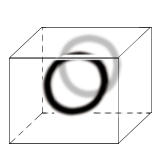
\includegraphics[width=4cm]{inudos/cubo1.png}
  	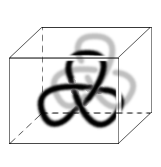
\includegraphics[width=4cm]{inudos/cubo2.png} 
  	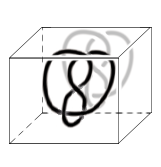
\includegraphics[width=4cm]{inudos/cubo3.png}
  	\centering
  	\caption{De izquierda a derecha: nudo trivial, nudo trébol, nudo de ocho.}
  	\label{trid} 
  \end{figure}

Nos interesa saber cuándo dos nudos son equivalentes: se puede pasar de uno a otro mediante deformaciones. Veámoslo formalmente:\\

Se dice que dos nudos son equivalentes si existe un homeomorfismo de  $\mathds{R}^{3}$ que nos lleve de un nudo al otro. \\


Podemos representar un nudo en el plano visualizando su proyección. Como hay muchas formas de representar un mismo nudo, podremos tener diferentes proyecciones que representen al mismo nudo. 
 Algunos ejemplos básicos son los siguientes:\\
  \begin{figure}[h!]
  	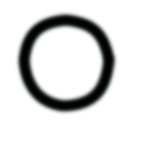
\includegraphics[width=3cm]{inudos/1.jpg}
  	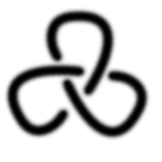
\includegraphics[width=3cm]{inudos/3f.png} 
  	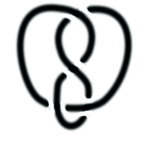
\includegraphics[width=3cm]{inudos/fig8.jpg}
  	\centering
  	\caption{Proyecciones del nudo trivial, nudo trébol, nudo de ocho.}
  	\label{uno} 
  \end{figure}
  
  Podemos ver en ellos una serie de cruces. En concreto en el nudo trébol tenemos 3 cruces y el nudo de ocho tenemos 4 cruces. El nudo trivial destaca por no tener ningún cruce. \\
  
    \underline{\textbf{Definición:}}\\
     Un \textbf{enlace} es una o más curvas cerradas disjuntas en $\mathds{R}^{3}$. Cada una de sus curvas recibe el nombre de componente.\\
     Por ejemplo, el siguiente enlace tiene dos componentes:
  \begin{figure}[h!]
  	
\includegraphics[width=2.7cm]{inudos/enlace.png}
  	\centering
  	\label{dos} 
  \end{figure}

    Por tanto, podemos ver un nudo como un caso particular de enlace en el que sólo tenemos una componente.\\
    
  Una de las cuestiones más interesantes en la teoría de nudos es la siguiente: \\
  ¿Dada un nudo, o alguna proyección suya, podremos saber si se trata del nudo trivial?. A lo largo de este proyecto trataremos de dar respuesta, en parte, a dicha cuestión.\\
  
 
  \newpage
\subsection{Sobre su historia y aplicaciones.}
En el siglo XIX, ciertos físicos escoceses se preguntaban por la estructura de los átomos.\\
Estos científicos tomaron como base la teoría de Descartes, que afirmaba que el \textit{éter} era un fluido que ocupaba todo el espacio y transmitía la luz (éter lumínico), para desarrollar su modelo del átomo. \\
Aunque dichos físicos conocían la existencia de los elementos y que estaban formados por átomos, no conocían la propia estructura de los átomos. \\

Científicos como Peter Guthrie Tait y Willian Thomson llegaron a la teoría de que los átomos se concebían como vórtices, que podríamos ver como remolinos tubulares, en dicho fluido. Estos vórtices se encontraban anudados y en función del tipo de anudamiento darían lugar a un tipo de elemento u otro.\\
De este modo se plantearon que los diferentes nudos corresponderían a los diferentes elementos de la naturaleza. De acuerdo con la teoría, si conociésemos todos los nudos posibles, crearíamos la tabla de elementos que reemplazaría la tabla periódica actual. \\

Para hacernos una idea más clara, para Willian Thomson el nudo trébol podría corresponder con el átomo de helio, el nudo de ocho con el átomo de oxígeno....\\

Numerosos científicos contribuyeron a dicha teoría intentando crear la tabla de nudos pero a finales de este mismo siglo, Michelson-Morley demostró que el éter lumínico no existía y por tanto la teoría de los átomos de vórtice fue descartada. \\

Tras este hecho, la teoría de nudos perdió su interés hasta que fue objeto de estudio en Topología a principios del siglo XX.\\

Posteriormente esta rama de la topología de baja dimensión destacó por su gran interés en áreas como:
  \begin{enumerate}
  	\item Química: ya hemos visto que la teoría de nudos nace en este área.
  	\item Biología: se estudia la teoría de nudos en la estructura de ADN.\\
  	Conocemos como ácido desoxirribonucleico (ADN) a aquella molécula que se encuentra en el núcleo de nuestras células y, por tanto, que contiene nuestro código genético. Se trata de un elemento esencial para la vida. Es muy conocida su forma: se puede ver como dos cuerdas enrolladas formando un doble hélice. \\
  	
  	Su forma de doble hélice puede encontrarse cerrada por los extremos de forma que nos encontraríamos con la propia forma de un nudo. Las ideas que veremos en este proyecto, junto con algunas más, se pueden aplicar a estas estructuras de ADN.\\
  	
  	Además, esta estructura de ADN puede sufrir ciertas alteraciones producidas por la encima topoisomerasa. Lo interesante es que estas alteraciones se corresponden con algunos de los movimientos que veremos para los nudos.\\
  	
  	
  	\item Criptografía: 
  	La fuerte relación que veremos entre la teoría de nudos y la teoría de trenzas, hace que podamos establecer cierta relación entre la teoría de nudos y la criptografía. \\
  	
  	Haciendo uso de la criptografía tratamos de encontrar métodos para que el intercambio de información no sea comprensible por terceras personas.\\
  	
  	Algunos métodos para encriptar dicha información están inspirados en la teoría de trenzas. En concreto el problema de la conjugación de trenzas, que trata de estudiar la igualdad de dos trenzas haciendo uso de una tercera trenza, nos permitirá encriptar la información de forma segura. \\
  \end{enumerate}

\newpage
\subsection{Componiendo nudos.}\label{seccion3}
Supongamos que tenemos dos proyecciones J y K de nudos. Podemos definir un nuevo nudo a partir de ellos eliminando un arco de cada una de las proyecciones y conectando los 4 extremos finales de dos en dos mediante otros arcos de modo que no se añadan ni eliminen cruces.\\
A este nudo resultante le llamaremos \textbf{suma conexa} o composición de los dos nudos y se denotará como \textbf{J\#K}. A los nudos originales J y K les llamaremos \textbf{nudos factores}. \\

Por ejemplo, consideremos como nudos factores el nudo trébol y el nudo de ocho. 
  \begin{figure}[h!]
  	\subfigure[J]{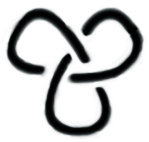
\includegraphics[width=2.5cm]{inudos/conexion1.jpg}} 
  	\subfigure[K]{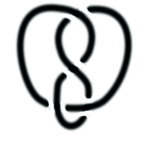
\includegraphics[width=2.5cm]{inudos/fig8.jpg}}
  	\centering
  	\caption{Nudo trébol y nudo de ocho.}
  	\label{comp1} 
  \end{figure}
  
Haciendo la suma conexa de ambos nudos obtenemos el nudo composición:
  \begin{figure}[h!]
  	\subfigure[Haciendo la composición]{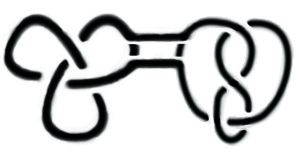
\includegraphics[width=7cm]{inudos/conexion2.jpg} }
  	\subfigure[J\#K]{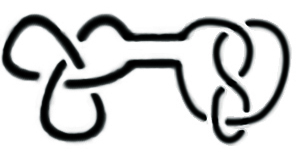
\includegraphics[width=7cm]{inudos/conexion3.jpg}}
  	\centering
  	\caption{Composición de nudo trébol y nudo de ocho.}
  	\label{comp2} 
  \end{figure}
  
  
  El nudo trivial es un elemento identidad para la suma conexa: si hacemos la composición de un nudo cualquiera J con el nudo trivial, vamos a obtener el propio nudo J. Por ejemplo, seguimos considerando J como el nudo trébol y el nudo trivial como K. \\
   \begin{figure}[h!]
   	\centering
   	\subfigure[J]{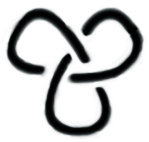
\includegraphics[width=2.5cm]{inudos/conexion1.jpg} }
   	\subfigure[K]{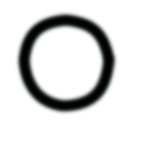
\includegraphics[width=2.5cm]{inudos/1.jpg}}
   	\caption{Nudo trébol y nudo trivial.}
   	\label{comp3} 
   \end{figure}
   
  Su suma conexa nos seguiría dando el nudo factor J, es decir, el nudo trébol.\\
   
      \begin{figure}[h!]
      	\subfigure[Haciendo la composición]{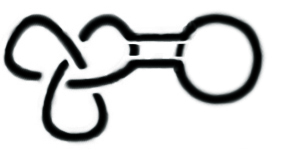
\includegraphics[width=8cm]{inudos/conexion4.jpg} }
      	\subfigure[J\#K]{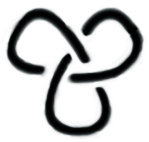
\includegraphics[width=4cm]{inudos/conexion1.jpg}}
      	\centering
      	\caption{Composición de nudo trébol y nudo trivial.}
      	\label{comp4} 
      \end{figure}
  
 \underline{\textbf{ Definición:}}\\
 Diremos que un \textbf{nudo es primo} si no puede ser expresado como la suma conexa de dos nudos, a menos que uno de ellos sea el nudo trivial. \\
 
\underline{ \textbf{ Definición:}}\\
 Diremos que un \textbf{nudo es compuesto} si no es el nudo trivial ni es un nudo primo.\\
  
  Por ejemplo, los nudos trébol y nudo de ocho de la figura \ref{comp1} son nudos primos mientras que el nudo de la figura \ref{comp2} es un nudo compuesto. \\ 
  
  Hay una gran variedad de nudos primos. Cualquier nudo puede ser expresado singularmente como suma conexa de nudos primos. En la siguiente tabla podemos ver los diferentes nudos primos que tienen menos de 8 cruces.\\
        \begin{figure}[h!]
        	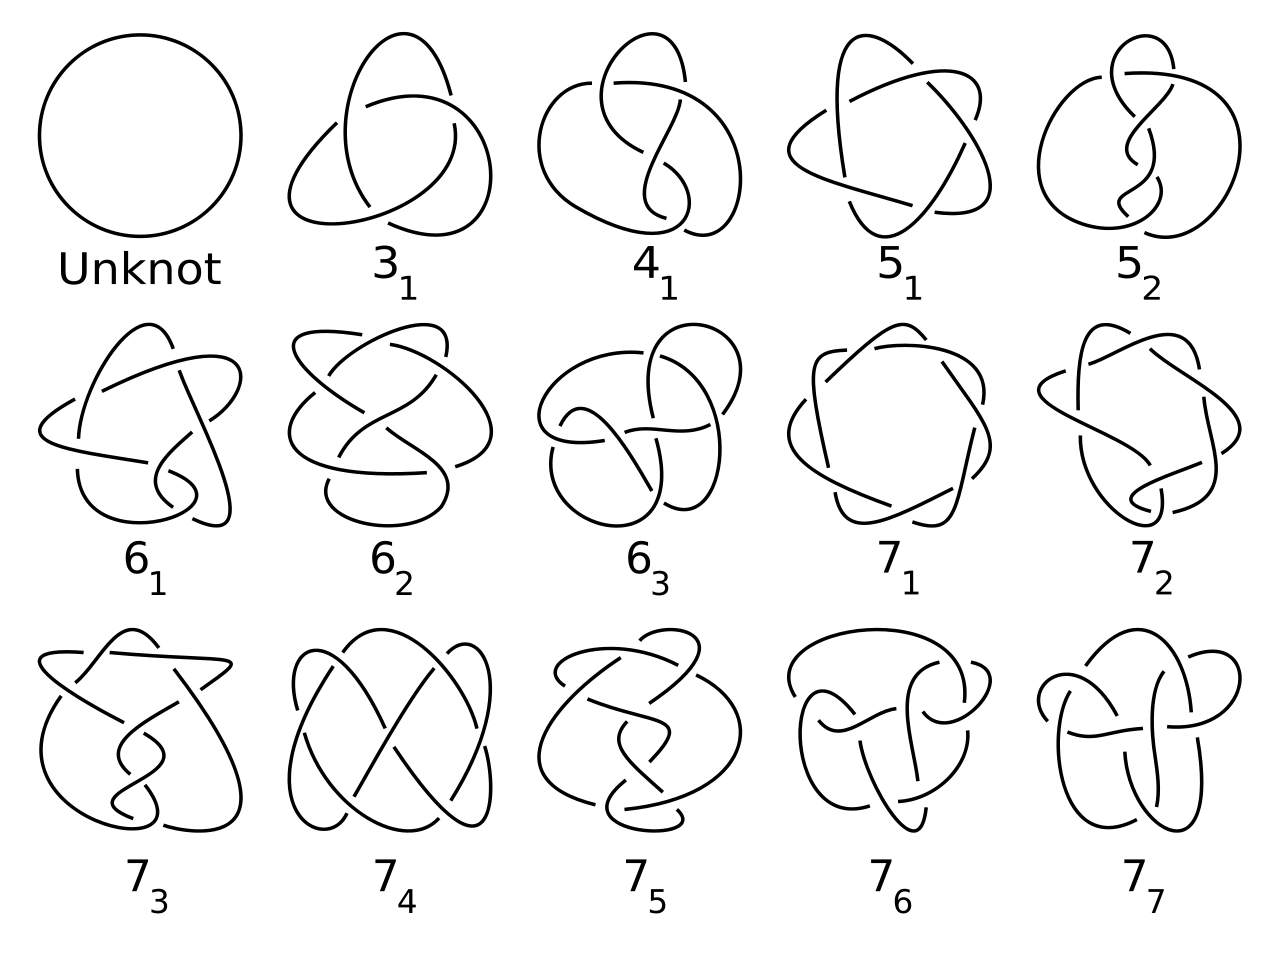
\includegraphics[width=14cm]{inudos/tableknot.png}
        	\centering
        	\caption{Composición de nudo trébol y nudo trivial.}
        	\label{comp6} 
        \end{figure}
  
  
  
    
    Finalmente, es importante destacar el hecho de que la elección que hacemos de los arcos que eliminamos de cada uno de los nudos factores afecta al nudo composición. Por tanto, es posible construir dos nudos composición diferentes a partir del mismo par de nudos factores. Veamos esta idea con más detalle, para ello necesitamos:\\
    
   \underline{\textbf{ Definición:}}\\
   \textbf{ Un nudo orientado} es un nudo al que se le ha asignado una orientación, es decir, es un nudo que dispone de una dirección de viaje sobre él mismo. Esta orientación se indica mediante flechas en la proyección. \\
   
   \underline{\textbf{ Definición:}}\\
   \textbf{ Un nudo es invertible} si es equivalente a sí mismo con la orientación opuesta. \\
   
      El problema de determinar si un nudo cualquiera es o no invertible no es para nada trivial.\\
   
   Como ejemplo de nuevo invertible nos podemos encontrar el nudo trébol.
      \begin{figure}[h!]
      	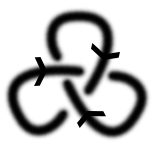
\includegraphics[width=3cm]{inudos/3fcon1.png}
      	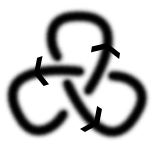
\includegraphics[width=3cm]{inudos/3fcon2.png}
      	\centering
      	\caption{Ambas orientaciones del nudo trébol.}
      	\label{comp5} 
      \end{figure}
   
   Sean los dos nudos factores J y K a los que se asignamos una orientación. Tendremos dos formas posibles de hacer la composición: conectar con las orientaciones emparejadas o no emparejadas. \\
   Todas las composiciones de los nudos cuyas orientaciones emparejan al componer, darán el mismo nudo composición. Todas las composiciones de los nudos cuyas orientaciones no emparejan al componer, también darán el mismo nudo composición. Sin embargo, es posible que la composición de los nudos cuyas orientaciones emparejen no de lugar al mismo nudo que haciendo la composición de los nudos cuyas orientaciones no emparejen. Serán el mismo si uno de los nudos factores es invertible.\\
   
   Veamos un caso en el que la composición de dos mismos factores, genera nudos diferentes. Consideramos el siguiente nudo:\\
   
         \begin{figure}[h!]
         	
\includegraphics[width=3cm]{inudos/817con.png}
         	\centering
         	\caption{Nudo factor J y K.}
         	\label{comp7} 
         \end{figure}
   Si componemos el nudo consigo mismo conectando las orientaciones emparejadas y desemparejadas obtenemos nudos que no son equivalentes. Lo podemos comprobar visualmente con la Figura \ref{comp8}.
   
         \begin{figure}[h!]
         	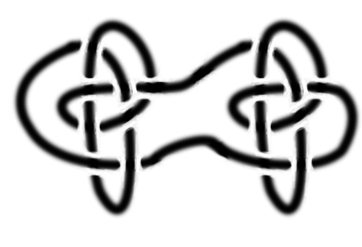
\includegraphics[width=6.5cm]{inudos/817def1.png}
         	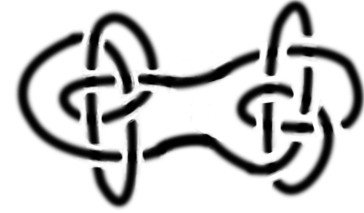
\includegraphics[width=6.5cm]{inudos/817def2.png}
         	\centering
         	\caption{Las composiciones no son equivalentes.}
         	\label{comp8} 
         \end{figure}
 
    
   
\subsection{Equivalencia de nudos: movimientos de Reidemeister.}\label{seccion4}
Dos nudos K1 y K2 serán equivalentes (K1 $\thicksim$ K2) si podemos distorsionar uno de ellos en el otro sin hacer ningún corte. \\

Para ver si dos proyecciones corresponden a nudos equivalentes, usaremos el conepto de isotopía plana. Más precisamente, definimos una \textbf{isotopía plana} de las proyecciones P1 y P2 de nudos como la aplicación continua $F: \mathds{R}^{2}$ x $[0,1] \rightarrow \mathds{R}^{2}$ tal que $F_{0}=identidad$, $F_{1}(P1) = P2$ y $F_{t}$ es un homeomorfismo $\forall t$.\\

Los movimientos de Reidemeister que vamos a ver a continuación nos permiten cambiar la proyección de un nudo de modo que se cambie la relación entre los cruces pero que no cambie el nudo al que representa la proyección. Cada uno de estos movimientos es una isotopía:\\

	\textbf{Primer movimiento de Reidemeister - R1}\\
En cualquier zona de la proyección nos permite añadir o eliminar un giro tal y como vemos en la figura \ref{movi1}.\\

  \begin{figure}[h!]
  	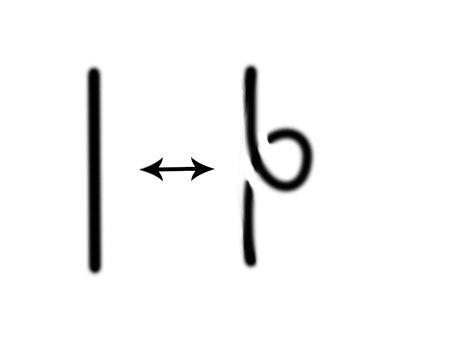
\includegraphics[width=7.2cm]{inudos/movi1.png}
  	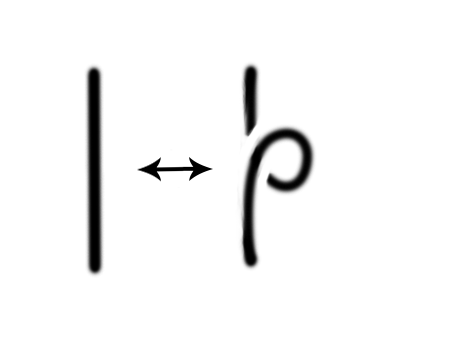
\includegraphics[width=7.2cm]{inudos/movi2.png}
  	\centering
  	\caption{Primer movimiento Reidemeister.}
  	\label{movi1} 
  \end{figure}
  
	\textbf{Segundo movimiento de Reidemeister - R2.}\\
Nos permite añadir o eliminar dos cruces del nudo como se ve en la figura \ref{movi2}.\\

    \begin{figure}[h!]
    	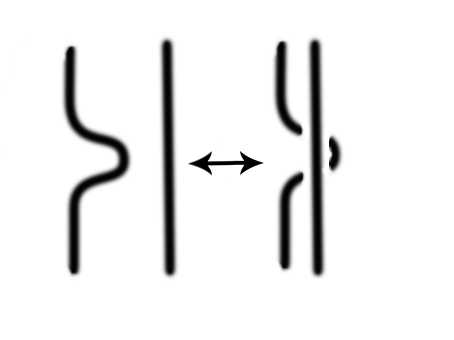
\includegraphics[width=7.5cm]{inudos/movi3.png}
    	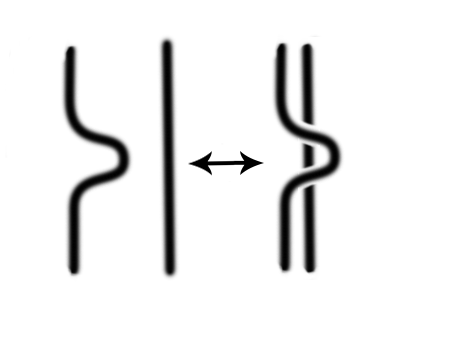
\includegraphics[width=7.5cm]{inudos/movi4.png}
    	\centering
    	\caption{Segundo movimiento de Reidemeister.}
    	\label{movi2} 
    \end{figure}
    
	\textbf{Tercer movimiento de Reidemeister - R3.}\\
Nos permite deslizar una hebra del nudo de un lado de un cruce al otro lado del cruce. Veamos la figura \ref{movi3} para aclarar la idea.
      \begin{figure}[h!]
      	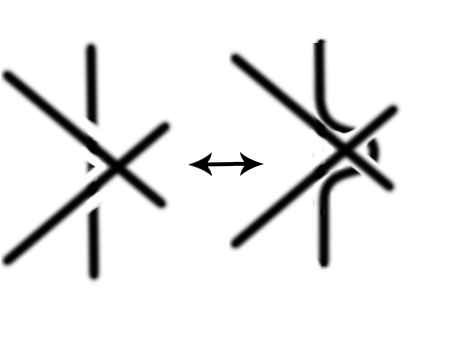
\includegraphics[width=7.5cm]{inudos/movi5.png}
      	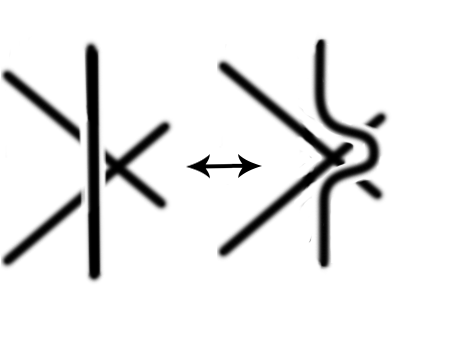
\includegraphics[width=7.5cm]{inudos/movi6.png}
      	\centering
      	\caption{Tercer movimiento de Reidemeister.}
      	\label{movi3} 
      \end{figure}
  

\begin{teo} \textbf{Teorema de Reidemeister.} Sean P1 y P2 las proyecciones que representan a dos nudos K1 y K2, respectivamente. Entonces, K1 $\thicksim$ K2 si, y solo si, P1 y P2 están conectados por una secuencia finita de movimientos de Reidemeister e isotopías planas.
\end{teo}
//AUN PENDIENTE DEMOSTRACIÓN.\\

Veamos un ejemplo en el que vemos la equivalencia de dos proyecciones, que en un primer momento podrían no parecernos equivalentes:
  \begin{figure}[h!]
  	\subfigure[P1]{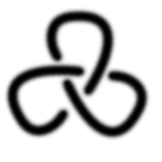
\includegraphics[width=3cm]{inudos/3f.png}}
  	\subfigure[R1]{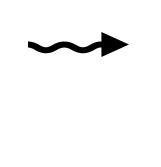
\includegraphics[width=2cm]{inudos/flecha.png}}
  	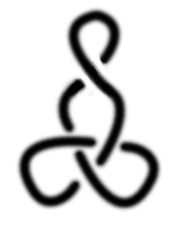
\includegraphics[width=3cm]{inudos/3fseg.png}
  	\subfigure[R3]{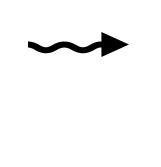
\includegraphics[width=2cm]{inudos/flecha.png}}
  	
\includegraphics[width=3cm]{inudos/fase3.png}
  	\subfigure[Isotopia]{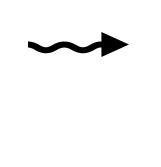
\includegraphics[width=2cm]{inudos/flecha.png}}
  	
\includegraphics[width=3cm]{inudos/fase4.png}
  	\subfigure[R3]{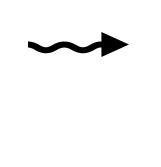
\includegraphics[width=2cm]{inudos/flecha.png}}
  	
\includegraphics[width=3cm]{inudos/fase5.png}
  	\subfigure[R1]{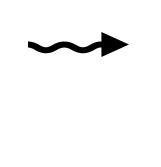
\includegraphics[width=2cm]{inudos/flecha.png}}
  	
\includegraphics[width=3cm]{inudos/fase6.png}
  	\subfigure[Isotopia]{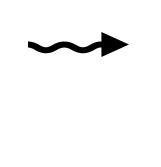
\includegraphics[width=2cm]{inudos/flecha.png}}
  	
\includegraphics[width=3cm]{inudos/fase7.png}
  	\subfigure[Isotopia]{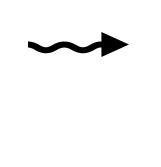
\includegraphics[width=2cm]{inudos/flecha.png}}
  	\subfigure[P2]{
\includegraphics[width=3cm]{inudos/fase8.png}}
  	\centering
  	\caption{Equivalencia de dos proyecciones de nudos.}
  	\label{algosj} 
  \end{figure}

Gracias a dicho teorema podremos estudiar si dos proyecciones representan el mismo nudo. Para ello tendremos que encontrar una secuencia de movimientos de Reidemeister que nos lleve de una proyección a la otra. Sin embargo, este proceso puede no tener el número de movimientos intermedios limitado por lo que no tiene mucho sentido implementarlo.\\
 
 Aunque este teorema no nos permita ver de una forma cómoda la equivalencia entre dos nudos en la práctica (por la fuerte complejidad) si que nos permite obtener una conclusión esencial:\\
 
 Si una propiedad de un nudo no cambia al aplicarle cualquiera de estos tres movimientos de Reidemeister, entonces esta propiedad no va a cambiar por muchas deformaciones que se le hagan al nudo. En definitiva, si un nudo cumple cierta propiedad y otro nudo no la cumple, esos nudos no podrán ser equivalentes. Incidiremos en esta idea en la siguiente Sección \ref{seccion5}.
 
  

\newpage
\subsection{Algunos invariantes.}\label{seccion5}
Suponga que cierto día ha ido a trabajar con su portátil fuera de casa y se lo ha dejado olvidado. Cuando te das cuenta, vuelves a buscarlo pero ya no está. Pasan unos días y un amigo te comenta que se ha encontrado un portátil con $x$ número de puertos, procesador $y$ y modelo $z$.\\

Es claro que si alguna de esas características no fuese la de tu portátil, tendrías claro que no es el tuyo. Pero resulta que tu portátil tiene exactamente las mismas características. Piensas que tal vez sea tu portátil pero no tienes garantía de que realmente lo sea. \\

Algo similar, aplicado a nudos, es lo que vamos a tratar de ver en esta sección. ¿Dadas dos proyecciones, podremos decir que representan al mismo nudo? Vamos a tratar de estudiar ciertos invariantes sobre los nudos. Al igual que ocurría con el caso del portátil, si dos proyecciones tienen valores de un invariante distintos podremos decir que no representan al mismo nudo. Sin embargo, si ambos tienen valores de un invariante iguales no podremos saber si se trata del mismo nudo. Tendremos que estudiar otros invariantes de nudos. \\

¿Y si estudiamos una gran cantidad de invariantes de dos proyecciones y siempre toman los mismos valores?¿Podremos garantizar que son equivalentes? La respuesta es clara, no. Tendremos que analizar en mayor detalle las proyecciones, pero puede ser que no lleguemos a obtener un conclusión definitiva. \\

    
Por tanto, el estudio de invariantes de los nudos nos va a permitir saber si dos nudos pueden ser (destacamos, que no quiere decir que lo sean) o no son equivalentes.\\


Antes de ver algunos de los invariantes de nudos más conocidos y útiles vamos a dar una definición formal de lo que se conoce como un invariante:\\

\underline{\textbf{Definición:}} \\
Un \textbf{invariante} de un nudo (o de un enlace) es una propiedad que no cambia cuando el nudo sufre deformaciones en el espacio. \\



\begin{center}
	\subsubsection{Número de componentes:}
\end{center}
Es uno de los invariantes de enlaces más sencillos que nos podemos encontrar y que ya hemos comentado ligeramente en las secciones anteriores.\\

Cada componente de un enlace es una curva disjunta del mismo. En la Figura \ref{inv1} vemos un enlace con dos componentes. 
  \begin{figure}[h!]
  	
\includegraphics[width=2.7cm]{inudos/enlace.png}
  	\centering
  	\caption{Enlace con dos componentes.}
  	\label{inv1} 
  \end{figure}
  
Al aplicarle a un enlace cualquier transformación no se le puede añadir ni eliminar ninguna componente. De modo que este invariante no nos va a permitir comparar nudos, pues todo nudo tiene una sola componente. \\

\bigskip
\begin{center}
	\subsubsection{Crossing number:}
\end{center}
Sea un nudo K. Su \textbf{crossing number} es el menor número de cruces que se encuentra en cualquier proyección del nudo. Se denota como $c(K)$. \\

Esto nos lleva a deducir el nudo K tendrá como mínimo c(K) cruces por muchas transformaciones que se haga a sus proyecciones.\\

Aunque es un invariante sencillo de visualizar, no es fácil de obtener: puede ser que al estudiar muchas proyecciones de un nudo pensemos que su número de cruces es $n$, sin embargo pueden existir otras proyecciones del nudo que no conocemos con menor número de cruces. Por este motivo, no vamos a trabajar posteriormente con este invariante.\\

Para dejarlo más claro vamos a ver un ejemplo.\\
Consideramos la proyección de la primera figura \ref{cross1}. Podemos pensar que el número de cruces del nudo sería 4 (ver los 4 cruces de la figura a). Sin embargo, esta proyección es equivalente a la proyección que vamos en la figura b, que tiene como número de cruces el valor 3. Por tanto, el número de cruces del nudo, que es el nudo trébol, es 3. 
   \begin{figure}[h!]
   	\centering
   	\subfigure[4 cruces]{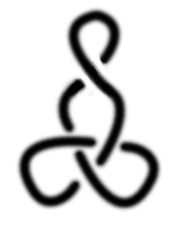
\includegraphics[width=3.5cm]{inudos/3fseg.png}}
   	\subfigure[3 cruces]{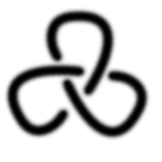
\includegraphics[width=3.5cm]{inudos/3f.png}}
   	\caption{Crossing number del nudo trébol.}
   	\label{cross1} 
   \end{figure}  


\begin{center}
	\subsubsection{Tricolorabilidad:}
\end{center}
Para definir este invariante de enlaces, tenemos que conocer unos conceptos previos:\\
Entendemos por undercrossing y overcrossing a un recorrido en el cruce de la proyección de un nudo que nos lleva por encima o por debajo en el cruce. Veamos la siguiente imagen donde queda representado:\\
   \begin{figure}[h!]
   	\centering
   	
\includegraphics[width=6.5cm]{inudos/cruce.png}
   	\caption{Tipo de cruce.}
   	\label{tric1} 
   \end{figure}

\underline{\textbf{Definición:}}\\
Una\textbf{ hebra }de una proyección de un enlace es una región de cuerda del enlace que va desde un undercrossing a otro undercrossing atravesando sólo overcrossings.\\ 

\underline{\textbf{Definición:}}\\
Una proyección de un enlace es tricolorable si cada una de las hebras de la proyección puede ser coloreada con uno de tres colores diferentes de modo que en cada cruce o los 3 colores se junten o se junte un sólo color. En este caso diremos que el enlace es \textbf{tricolorable}. 

\begin{teo}
	La tricolorabilidad se perserva mediante movimientos de Reidemeister.
\begin{proof}
	Supongamos que partimos de una proyección de un nudo que es tricolorable y vamos a aplicarle los movimientos de Reidemeister. Tendremos que ver que la proyección final es tricolorable. Podemos centrarnos en la zona de la proyección a la que se le aplica el movimiento. Veamos qué ocurre al aplicar cada movimiento:\\
	
	\underline{R1:}
	En este caso sólo se puede dar que tengamos un sólo color. Al aplicar el movimiento R1 seguiremos utilizando ese mismo color, de modo que la proyección modificada seguirá siendo tricolorable. 
	   \begin{figure}[h!]
	   	\centering
	   	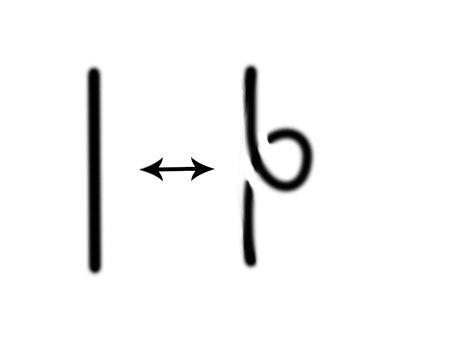
\includegraphics[width=4cm]{inudos/movi1.png}
	   	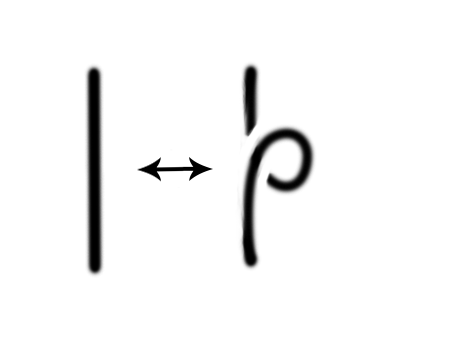
\includegraphics[width=4cm]{inudos/movi2.png}
	   	\caption{}
	   	\label{demotri1} 
	   \end{figure}
	   
	\underline{R2:}
	Supongamos que el coloreado inicial se ha realizado con un sólo color. Al igual que con el movimiento R1, no tendríamos ninguna dificultad pues al aplicar el movimiento R2 seguiremos coloreando con el mismo color y la proyección seguirá siguiendo tricolorable. \\
	\begin{figure}[h!]
		\centering
		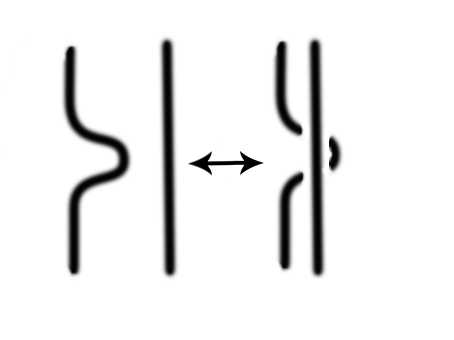
\includegraphics[width=4cm]{inudos/movi3.png}
		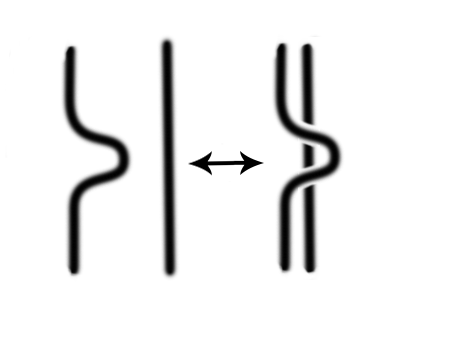
\includegraphics[width=4cm]{inudos/movi4.png}
		\caption{}
		\label{demotri2} 
	\end{figure}
	
	Ahora tenemos otra segunda opción de coloreado en la proyección inicial y es que en ambos cruces posibles usemos los 3 colores posibles. Se puede ver en la figura \ref{demotri3}. Se observa que la proyección sigue siendo tricolorable. \\
	
	\begin{figure}[h!]
		\centering
		\includegraphics[width=8cm]{inudos/movi3tri.png}
		\includegraphics[width=8cm]{inudos/movi4tri.png}
		\caption{}
		\label{demotri3} 
	\end{figure}
	
		\underline{R3:}
	Este movimiento tiene más complejidad pues tenemos 3 cruces posibles. Analizamos todos los casos posibles y vemos que nos podemos reducir a cinco situaciones. Veamos en la figura \ref{demotri4} cómo sería el cambio de color en cada caso para confirmar que las proyecciones resultantes al aplicar el movimiento siguen siendo tricolorables. \\
		\begin{figure}[h!]
			\centering
			\includegraphics[width=8cm]{inudos/movi5.png}
			\includegraphics[width=8cm]{inudos/movi5tri1.png}
			\includegraphics[width=8cm]{inudos/movi5tri2.png}
			\includegraphics[width=8cm]{inudos/movi5tri3.png}
			\includegraphics[width=8cm]{inudos/movi5tri4.png}
			\caption{}
			\label{demotri4} 
		\end{figure}
		
	Concluimos que si tenemos una proyección tricolorable y aplicamos los movimientos de Reidemeister, la proyección resultante sigue siendo tricolorable. \\
	Si la proyección de partida no fuese tricolorable, la proyección resultante tampoco podría ser tricolorable: supongamos que la proyección resultante es tricolorable, por el razonamiento que hemos seguido anteriormente, tendríamos que tener que la proyección inicial sería tricolorable llegando a contradicción. 
		
\end{proof}
\end{teo}


Haciendo uso de este invariante podemos demostrar que el nudo trivial y el nudo trébol no son equivalentes, es decir, son topológicamente distintos. Esto se debe a que el nudo trébol es tricolorable pero el nudo trivial no lo es. Podemos verlo en la imagen \ref{Tric2}:\\
   \begin{figure}[h!]
   	\centering
   	\subfigure[No tricolorable]{\includegraphics[width=5cm]{inudos/1.jpg}}
   	\subfigure[Tricolorable]{\includegraphics[width=5cm]{inudos/3ftri.png}}
   	\caption{Dos nudos no equivalentes.}
   	\label{Tric2} 
   \end{figure} 


Este hecho confirma que existe al menos un nudo distinto del nudo trivial. Es más, todo nudo que sea tricolorable será distinto del nudo trivial.\\

Sin embargo, este invariante no es muy potente en el sentido de que sólo clasifica los enlaces en tricolorables y no tricolorables y sólo podremos afirmar que dos proyecciones representan a diferentes nudos si una de ellas es tricolorable y la otra no lo es.   


\bigskip
\begin{center}
	\subsubsection{Unknotting number:}\label{subunk}
\end{center}
Supongamos que tenemos la proyección de un nudo no trivial. Modificar la proyección para que un undercrossing pase a ser un overcrossing, o viceversa, no es un movimiento válido pues estamos intersecando la cuerda. Sin embargo, es un movimiento interesante ya que nos llevará al nudo trivial. \\

\underline{\textbf{Definición:}}
Se define el \textbf{número de desanudamiento} de un nudo como el menor número de cambios en los cruces necesarios para desanudarlo, es decir, para llegar al nudo trivial. Se denota como $u(K)$. \\

Es claro que en un número finito de pasos conseguiremos obtenemos el número de desanudamiento: Recorremos el nudo con cierta orientación y al llegar a un cruce, si no hemos pasado anteriormente por él y es un undercrossing, lo convertimos en overcrossing. \\ 

Podemos ver, en la figura \ref{unk1}, que el número uno es el número de desanudamiento para el nudo trébol. El punto de partida lo indicamos con un punto grueso.
   \begin{figure}[h!]
   	\centering
   	\subfigure[Nudo de partida]{\includegraphics[width=4cm]{inudos/3fcon1start.png}}
   	\subfigure[Nudo modificado]{\includegraphics[width=4cm]{inudos/3fcon1negstart.png}}
   	\caption{Unknotting number trébol.}
   	\label{unk1} 
   \end{figure}

\bigskip
\begin{center}
	\item \subsubsection{Polinomio de Alexander:}\label{alenudos}
\end{center}
Anteriormente hemos visto algunos invariantes geométricos y numéricos que nos pueden ayudar en la tarea de comprobar si dos proyecciones representan al mismo nudo. Ahora vamos a ver un invariante polinómico que estudiaremos con más detalle pues será uno de los puntos fuertes que implementaremos para resolver, en parte, la cuestión. \\

Se trata de un polinomio, con variable $t$, para nudos orientados. En 1969, se probó que dicho polinomio puede calcularse computacionalmente haciendo uso de dos reglas:
\begin{itemize}
	\item \underline{Regla 1:} \\
	El polinomio de Alexander del nudo trivial es el polinimio trivial equivalente a 1. Esta regla se representa como $\vartriangle$($\bigcirc$)= 1
\end{itemize}

Para poder exponer la segunda regla tenemos que conocer antes las siguientes ideas. \\
Consideramos el enlace orientado de partida. Si nos centramos en uno de sus cruces, podemos crear tres nuevos enlaces orientados exactamente iguales al de partida variando únicamente en este cruce seleccionado. A cada uno de estos nuevos enlaces le establecemos uno de estos nuevos cruces:
\begin{enumerate}
	\item $L_{+}$: El cruce seleccionado se establece como positivo.
	\item $L_{-}$: El cruce seleccionado se establece como negativo.
	\item $L_{0}$: El cruce seleccionado se elimina.
\end{enumerate}
Podemos ver estos nuevos cruces en la figura \ref{alex1}.\\

   \begin{figure}[h!]
   	\centering
   	\subfigure[$ L_{+} $]{\includegraphics[width=4cm]{inudos/pro1.png}}
   	\subfigure[$ L_{-} $]{\includegraphics[width=4cm]{inudos/pro2.png}}
   	\subfigure[$ L_{0} $]{\includegraphics[width=4cm]{inudos/pro3.png}}
   	\caption{Tipos de cruces.}
   	\label{alex1} 
   \end{figure}


\begin{itemize}
	\item \underline{Regla 2:} \\
	 Esta regla se representa como $\vartriangle(L_{+}) - \vartriangle(L_{-}) +  (t^{\frac{1}{2}} - t^{\frac{-1}{2}}) \vartriangle(L_{0})  = 0$
\end{itemize}

Veamos cómo se calcularía el polinomio de Alexander con el nudo trébol:\\
Como el nudo de partida tiene más de un cruce, tenemos que aplicarle la segunda regla. Consideraremos como cruce a cambiar el que nos encontramos más a la izquierda aunque podríamos considerar cualquier otro cruce. Generamos los tres nuevos enlaces haciendo el cambio en el cruce. Sus proyección se pueden ver en la figura \ref{alex2}. Las llamamos A, B y C por comodidad. 
   \begin{figure}[h!]
   	\centering
   	\subfigure[A]{\includegraphics[width=4cm]{inudos/3fcon1.png}}
   	\subfigure[B]{\includegraphics[width=4cm]{inudos/3fcon1neg.png}}
   	\subfigure[C]{\includegraphics[width=4cm]{inudos/doble1b.png}}
   	\caption{}
   	\label{alex2} 
   \end{figure}

Al aplicar la segunda regla tendremos:\\
\begin{equation}
 \vartriangle(A) - \vartriangle(B) +  (t^{\frac{1}{2}} - t^{\frac{-1}{2}}) \vartriangle(C)  = 0.
 \end{equation}
 Sabemos que $\vartriangle(B)$ = $\vartriangle$($\bigcirc$)= 1. Luego nos quedaría la ecuación:
\begin{equation}
\vartriangle(A) +  (t^{\frac{1}{2}} - t^{\frac{-1}{2}}) \vartriangle(C)  = 1.
\end{equation}
Ahora necesitamos conocer el valor de $\vartriangle(C)$. Al igual que ocurría anteriormente, la proyección de este nuevo nudo tiene más de un cruce de modo que vamos a aplicarle la segunda regla. Esta vez seleccionamos el cruce superior como cruce que se modifica en los nuevos nudos. Obtenemos las proyecciones que vemos en la figura \ref{alex3}, a las que llamaremos D y E. 
   \begin{figure}[h!]
   	\centering
   	\subfigure[D]{\includegraphics[width=4cm]{inudos/doble2b.png}}
   	\subfigure[E]{\includegraphics[width=4cm]{inudos/doble3b.png}}
   	\caption{}
   	\label{alex3} 
   \end{figure}

Al aplicar la segunda regla tendremos:\\
\begin{equation}
\vartriangle(C) - \vartriangle(D) +  (t^{\frac{1}{2}} - t^{\frac{-1}{2}}) \vartriangle(E)  = 0.
\end{equation}
 Sabemos que $\vartriangle(E)$ = $\vartriangle$($\bigcirc$)= 1. Además $\vartriangle(D)$ = $\vartriangle$($\bigcirc$ $\bigcirc$)= 0. Luego nos quedaría la ecuación:
 \begin{equation}
 \vartriangle(C) = -  (t^{\frac{1}{2}} - t^{\frac{-1}{2}}).
 \end{equation}

Volviendo a la ecuación (2) tendemos:
\begin{equation}
\vartriangle(A) =  (t^{\frac{1}{2}} - t^{\frac{-1}{2}})^{2} + 1 = t^{-1} -1 + t.
\end{equation}
Luego $ t^{-1} -1 + t $ es el polinomio de Alexander del nudo trébol. \\

\bigskip
Es importante destacar el hecho de que podemos tener un nudo no trivial que tenga como polinomio de Alexander el polinomio trivial equivalente a 1. Por este motivo, con dicho invariante no podemos distinguir cualquier nudo del nudo trivial. \\

¿Mediante estas dos reglas podremos obtener siempre el polinomio de Alexander en tiempo finito? La respuesta es afirmativa, veámoslo:\\

La idea que vamos a seguir en este proceso será reducir las proyecciones, a las que le queremos obtener el polinomio de Alexander, hasta llegar al nudo trivial. Reducir estas proyecciones quiere decir ir modificando sus cruces obteniendo $L_{+}$, $L_{-}$ y $L_{0}$ . Como veíamos en el invariante de la sección \ref{subunk}, a cualquier proyección le podemos aplicar una secuencia finita de cambios en los cruces de modo que resulte el nudo trivial. Por tanto, este procedimiento tendrá fin en una secuencia finita de pasos.\\

Al ir considerando los distintos nudos de la proyección, obtendremos dos nuevas proyecciones en cada paso. Con estas nuevas proyecciones podremos formar lo que se denomina \textbf{ árbol de resolución}. En la figura \ref{alex4} podemos ver el árbol de resolución del nudo trébol.\\

   \begin{figure}[h!]
   	\centering
   	\includegraphics[width=18cm]{inudos/arbol.png}
   	\caption{Árbol de resolución del nudo trébol.}
   	\label{alex4} 
   \end{figure}

\underline{\textbf{Definición:}}\\
Se define la \textbf{profundidad de un nudo} (o enlace) como el mínimo número de niveles que nos encontramos en los árboles de resolución del nudo. \\

Esta profundidad del nudo es un invariante que además nos permite medir la complejidad que supondrá el cálculo del polinomio de Alexander. \\

El árbol de resolución del nudo trébol que vemos en la figura \ref{alex4} tiene una profundidad de 2 niveles (la proyección inicial no se cuenta como nivel). Es importante destacar que el único nudo que tiene profundidad de nudo igual a 0 es el nudo trivial. \\
 
\newpage
\subsection{Notación de nudos.}
Ya sabemos qué son los nudos y algunas nociones esenciales sobre los mismos, pero aún no sabemos asociar una notación concreta a un nudo. En esta sección vamos a ver algunas de las notaciones más comunes de los nudos. 

\begin{center}
	\item \subsubsection{Notación de Dowker:}
\end{center}
Se trata de una notación muy sencilla para describir la proyección de un nudo. La notación en sí es una secuencia de números enteros, veamos cómo se obtiene:\\

Consideramos una orientación en la proyección de n cruces y asignamos el valor 1 al primer cruce que nos encontremos. Continuamos por la proyección y asignamos el valor 2 al siguiente cruce. Vamos repitiendo el proceso hasta pasar por cada cruce un par de veces (una vez por el undercrossing y otra por el overcrossing). Como resultado tendremos un número par y un número impar por cada cruce de la proyección. \\

Finalmente es necesario asignar los signos a cada uno de estos $2n$ números. Los números pares que correspondan a un overcrossing tendrán signo negativo. Veamos un ejemplo con el nudo trébol:\\
   \begin{figure}[h!]
   	\centering
   	\includegraphics[width=4cm]{inudos/3fcon2dow.png}
   	\caption{Numeración de cruces-Dowker.}
   	\label{dow1} 
   \end{figure}
   
  Tendríamos los pares (1,-4), (3,-6) y (5,2). La notación de Dowker sería -4 -6 2 pues nos quedamos únicamente con los números pares en el orden que indican los números impares.\\

\begin{center}
	\item \subsubsection{Notación de Gauss:}
\end{center}
La notación de Gauss es una notación parecida a la de Dowker. Consideremos de nuevo una orientación en la proyección de n cruces de un nudo.\\

En este caso cada vez que pasamos por un cruce, tendremos un solo número asignado. De este modo la secuencia de números de la notación se compone de $2n$ elementos con valores desde 1 hasta n, cada uno de ellos repetido dos veces.\\

Consideramos una orientación en la proyección de n cruces y asignamos el valor 1 al primer cruce que nos encontremos. Realizamos el siguiente proceso: continuamos por la proyección hasta el siguiente cruce. Si ya hemos pasado por él, anotamos el número de cruce que tenga asociado. Si no hemos pasado anteriormente por él, asignamos el siguiente número de cruce.\\

Finalmente es necesario asignar los signos a cada uno de esos $2n$ números. Los números que representen uncrossings tendrán signo negativo. Veamos la notación de Gauss para el nudo trébol.\\
   \begin{figure}[h!]
   	\centering
   	\includegraphics[width=4cm]{inudos/3fcon2gaus.png}
   	\caption{Numeración de cruces-Gauss.}
   	\label{gaus1} 
   \end{figure} 
Si vamos haciendo el recorrido partiendo desde el punto grueso indicado tendríamos la secuencia de números: -1 2 -3 1 -2 3. Esta sería su notación de Gauss.

\begin{center}
	\item \subsubsection{Notación de Conway:}
\end{center}
Por último vamos a ver una notación que puede resultar algo más compleja pero que tiene gran uso e interés, sobre todo en la tería del ADN. \\

\underline{\textbf{Definición:}}\\
Un \textbf{enredo} o tangle de una proyección de un enlace es una región de la proyección rodeada por una bola de modo que las dos cuerdas enlazadas de la proyección tocan la bola exactamente en cuatro puntos. A estos puntos los denotaremos como NO, NE, SO y SE.\\

En la figura \ref{conw1} vemos un enredo general y un ejemplo particular de un enredo.\\
   \begin{figure}[h!]
   	\centering
   	\subfigure[Enredo general]{\includegraphics[width=4cm]{inudos/en1.png}}
   	\subfigure[Ejemplo de enredo]{\includegraphics[width=4cm]{inudos/en2.png}}
   	\caption{}
   	\label{conw1} 
   \end{figure} 

Pero la idea es trabajar con enredos más sencillos como son los que vemos en la figura \ref{conw2}. La notación se corresponde con el número de cruces que tiene el enredo con signo positivo y negativo según se ve en las imágenes.\\
   \begin{figure}[h!]
   	\centering
   	\subfigure[Enredo $\infty$]{\includegraphics[width=4cm]{inudos/en3.png}}
   	\subfigure[Enredo 0]{\includegraphics[width=4cm]{inudos/3enrot.png}}
   	
   	\subfigure[Enredo 4]{\includegraphics[width=10cm]{inudos/en4.png}}
   	
   	\subfigure[Enredo -4]{\includegraphics[width=10cm]{inudos/en4conneg.png}}
   	\caption{Tipos básicos de enredos.}
   	\label{conw2} 
   \end{figure} 

Haciendo uso de estos enredos básicos podemos construir nuevos enredos uniendo, respectivamente, los extremos NE y SE de un enredo con los extremos NO y SO del otro enredo. A esta operación se le conoce como suma de enredos.\\
Además, disponemos de una operación de multiplicación: reflejaremos el primer enredo y hacemos la operación de suma.\\
A los enredos construidos con estas operaciones se les conoce con \textbf{enredos racionales}. Podemos ver un esquema básico estas dos operaciones en la imagen \ref{conw3}:\\
   \begin{figure}[h!]
   	\centering
   	\subfigure[Operacion suma]{\includegraphics[width=8.5cm]{inudos/ensum.png}}
   	\subfigure[Operacion multiplicacion]{\includegraphics[width=8.5cm]{inudos/enmul.png}}
   	\caption{Operaciones con enredos.}
   	\label{conw3} 
   \end{figure}

En la figura \ref{conw4} podemos ver un ejemplo de un enlace más complejo:
\begin{figure}[h!]
	\centering
	\includegraphics[width=3.5cm]{inudos/en5fin.png}
	\caption{Enlace -2 3 2}
	\label{conw4} 
\end{figure}

A partir de estos enredos podemos construir proyecciones de nudos enlazando los puntos NO con NE y los puntos SO con SE. La notación del nudo corresponde con la notación que le damos a su enredo.\\ 

Nos interesa ver si dos proyecciones de nudos representan al mismo nudo, luego nos interesa ver si dos enredos son equivalentes. Veamos qué quiere decir que sean equivalentes:\\

\underline{\textbf{Definición:}}\\
Diremos que dos enredos son equivalentes si podemos pasar de un enredo al otro mediante los movimientos de Reidemeister, que vimos en la sección \ref{seccion4}, manteniendo los cuatro extremos fijos en la bola imaginaria. \\

Ver si dos enredos son equivalentes por definición no es viable de modo que vamos a aplicar otro método: consiste en calcular la fracción continua asociada a cada enredo.\\

\underline{\textbf{Definición:}}\\
Sea un enredo con notación $a_{n}...a_{1}a_{0}$. Su\textbf{ fracción continua} es una expresión del tipo:
\begin{equation}
    a_{0} + \frac{1}{a_{1} + \frac{1}{a_{2} + \frac{1}{...a_{n}}}}
\end{equation}
siendo $a_{i} \in \mathds{Z},  \forall i = 0,1,..,n.$\\

\begin{teo}
Dos enredos racionales son equivalentes si y solo si sus fracciones continuas toman el mismo valor. 
\end{teo}

Veamos un ejemplo. Consideramos los enredos racionales -2 3 2 y 3 -2 3 que vemos en la siguiente figura.\\
\begin{figure}[h!]
	\centering
	\subfigure[Enlace -2 3 2]{\includegraphics[width=3.5cm]{inudos/en5fin.png}}
	\space
	\subfigure[Enlace 3 -2 3]{\includegraphics[width=3.5cm]{inudos/en6fin.png}}
	\caption{Enlaces equivalentes}
	\label{conw5} 
\end{figure}

A simple vista resulta difícil confirmar que sean equivalentes. Vamos a obtener sus fracciones continuas asociadas:\\
$-2 \hspace{1cm} 3 \hspace{1cm} 2 \hspace{1cm}$ tiene fracción continua
\begin{equation}
 2 + \frac{1}{3 + \frac{1}{-2}} = \frac{12}{5}
\end{equation}

$3 \hspace{1cm} -2 \hspace{1cm} 3 \hspace{1cm}$ tiene fracción continua
\begin{equation}
3 + \frac{1}{-2 + \frac{1}{3}} = \frac{12}{5}
\end{equation}
Ambas fracciones continuas son iguales, luego los enredos -2 3 2 y 3 -2 3 son equivalentes. 

\newpage
\subsection{Conexión con distintas teorías.}\label{seccion7}
\begin{center}
	\item \subsubsection{Teoría de grafos:}
\end{center}

\underline{\textbf{Definición:}}\\
Un \textbf{grafo} es un par $ (V,A) $ de conjuntos, junto con la aplicación 
\begin{center}
	 $  \gamma :A \rightarrow$ \{\{$u,v$\} / $u,v \in V$\}  
\end{center}
Al conjunto de puntos V se se llama conjunto de vértices y al conjunto A le llamaremos conjunto de aristas. \\

\underline{\textbf{Definición:}}\\
Un \textbf{grafo plano} $ G $ es un grafo que permanece en el plano.\\

Podemos ver varios ejemplos en la figura \ref{graf1}.\\
\begin{figure}[h!]
	\centering
	\includegraphics[width=3.5cm]{inudos/grafo.png}
	\includegraphics[width=4cm]{inudos/pgrafo.png}
	\caption{Ejemplos de grafos planos.}
	\label{graf1} 
\end{figure}

A partir de la proyección de un nudo (o de un enlace en general) podemos crear un grafo plano correspondiente. Para ello tendremos que realizar el siguiente proceso:\\

Sombreamos las regiones de la proyección que estén de modo que la región externa al nudo se quede sin sombrear y situamos un vértice en cada zona. Unimos los vértices con aristas que pasan por los cruces de la proyección. Ya tendríamos el grafo plano. Además, si el nudo tiene asignada una orientación, podremos asignarle el tipo de cruce (positivo o negativo) a cada arista. Podemos ver un ejemplo en la figura \ref{graf2}.\\
\begin{figure}[h!]
	\centering
	\includegraphics[width=5cm]{inudos/pgrafo3.png}
	\includegraphics[width=5cm]{inudos/pgrafo2.png}
	\includegraphics[width=5cm]{inudos/pgrafo1.png}
	\caption{De proyección a grafo}
	\label{graf2} 
\end{figure}

Finalmente, para ver que los problemas de nudos se pueden ver como problemas de grafos y viceversa, vamos a ver el procedimiento inverso. Dado un grafo plano, podremos obtener la proyección del nudo asociado. Veamos cuál sería el procedimiento:\\

Partiendo del grafo plano con los signos asociados en cada vértice, marcamos cada una de las aristas. Uniremos cada una de estas marcas con aquellas marcas que estén en las aristas que conectan con los vértices de la arista que tiene la marca. A continuación, sombreamos las zonas que contienen a cada vértice. Finalmente, establecemos los cruces conforme a los signos del grafo plano. Podemos ver un ejemplo en la figura \ref{graf3}.\\
\begin{figure}[h!]
	\centering
	\includegraphics[width=4.5cm]{inudos/grafo1.png}
	\includegraphics[width=4.5cm]{inudos/grafo2.png}
	\includegraphics[width=4.5cm]{inudos/grafo3.png}
	\includegraphics[width=4.5cm]{inudos/grafo4.png}
	\caption{De grafo a proyección.}
	\label{graf3} 
\end{figure}



\begin{center}
	\item \subsubsection{Teoría de trenzas:}
\end{center}
En esta sección vamos a introducir la relación que hay entre teoría de nudos y teoría de trenzas, teoría que estudiaremos con mayor detalle en el próximo tema.\\

Vamos a ver la idea general de lo que se entiende por el término trenza y veremos una definición más precisa más adelante. Podemos pensar en una trenza como un conjunto de $n$ cadenas que son atadas a un tope imaginario arriba y abajo. Podemos ver algunos ejemplos de trenzas en la figura \ref{ntren1}.\\
   \begin{figure}[h!]
   	\centering
   	\includegraphics[width=3.5cm]{itrenzas/t4.png}
   	\space
   	\includegraphics[width=6cm]{itrenzas/t7.png}
   	\caption{Ejemplos de trenzas}
   	\label{ntren1} 
   \end{figure} 

A partir de una trenza, podemos obtener su nudo o enlace correspondiente. Simplemente tendremos que unir en orden  los topes superiores de las cadenas con los inferiores. Esta trenza cerrada será el nudo al que representa la trenza. Podemos ver algunos ejemplos en la sección \ref{t2sec1}.\\

Para ver el proceso inverso haremos uso del siguiente teorema:
\begin{teo}Teorema de Alexander.\\
	Todo nudo puede ser representado como una trenza cerrada.
\end{teo}
//PENDIENTE DEMOSTRACIÓN A PARTIR DE POSIBLE IMPLEMENTACIÓN!!!!!!!!!!!!!!!!!!!!!


\newpage
\section{Teoría de trenzas. }\label{SegundoTema}
\subsection{Nudos y trenzas.}\label{t2sec1}
En la sección \ref{seccion7} dimos una idea general de lo que se entiende por una trenza. Veamos su definición más formal:\\

\underline{\textbf{Definición:}}\\
Consideremos el cubo $\mathds{D} = \{(x,y,z) / 0 \leq x,y,z \leq 1\}$ y situamos $A_{i}$ puntos en su cara superior y $B_{i}$ puntos en la cara inferior, siendo $i \in \mathds{N}$. Unimos cada punto $A_{i}$ con un punto $B_{i}$ mediante segmentos $d_{i}$ de modo que:
\begin{enumerate}
	\item $ d_{1}, d_{2},...,d_{n} $ sean disjuntos.
	\item Los segmentos $ d_{i} $ no pueden conectar puntos $A_{i}$ o $B_{i}$ entre sí.
	\item Al cortar por cualquier plano horizontal, cada segmento $ d_{i} $ toca en un sólo punto al plano. 
\end{enumerate}
A cada uno de estos segmentos $ d_{i} $ les llamaremos cadenas y al conjunto de las n-cadenas se le conoce como \textbf{trenza}.\\

Podemos ver algunos ejemplos de trenzas en la figura \ref{tren1}.\\
   \begin{figure}[h!]
   	\centering
   	\subfigure[$-\sigma2+\sigma1-\sigma2+\sigma1+\sigma3$]{\includegraphics[width=5cm]{itrenzas/t1cubo.png}}
   	\space
   	\subfigure[$+\sigma1-\sigma2+\sigma1-\sigma2$]{\includegraphics[width=5cm]{itrenzas/t2cubo.png}}
   	\caption{Ejemplos de trenzas}
   	\label{tren1} 
   \end{figure} 

Al igual que hacíamos con los nudos, podremos representar una trenza en el plano visualizando su proyección. En la figura \ref{tren2} se pueden ver las proyección de las trenzas representadas en la figura \ref{tren1}.\\
   \begin{figure}[h!]
   	\centering
   	\subfigure[$-\sigma2+\sigma1-\sigma2+\sigma1+\sigma3$]{\includegraphics[width=3cm]{itrenzas/t1pro.png}}
   	\space
   	\subfigure[$+\sigma1-\sigma2+\sigma1-\sigma2$]{\includegraphics[width=2.5cm]{itrenzas/t2pro.png}}
   	\caption{Proyección de trenzas}
   	\label{tren2} 
   \end{figure}  

Anteriormente vimos que a cada trenza le corresponde un nudo o un enlace particular. Se obtendrá uniendo los extremos superiores con los extremos inferiores de las cadenas en el mismo orden. A este nudo se le conocerá como \textbf{trenza cerrada}. \\

Denotaremos como $\mathscr{B}_{n}$ al conjunto de todas las trenzas de n cadenas.\\

 
\bigskip
\begin{center}
	\subsubsection{Notación de trenzas:}
\end{center}
Para poder trabajar de forma cómoda con las trenzas vamos a darle la siguiente notación:\\
Sean las cadenas que se encuentran en las posiciones $i$ e $i+1$. Al producir un intercambio de posiciones de estas cadenas se producirá un \textbf{cruce}. Este cruce puede realizarse de dos formas: 
\begin{itemize}
	\item La cadena que se encuentra en la posición $i$ cruza por delante de la cadena que inicialmente se encuentra en la posición $i+1$. En este caso el cruce se denota como $-\sigma(i)$.
	\item La cadena que se encuentra en la posición $i$ cruza por detrás de la cadena que inicialmente se encuentra en la posición $i+1$. En este caso el cruce se denota como $+\sigma(i)$.
\end{itemize}
Podemos verlo más claro en la figura \ref{tren4}.\\
   \begin{figure}[h!]
   	\centering
   	\subfigure[$-\sigma(i)$]{\includegraphics[width=3.5cm]{itrenzas/t5.png}}
   	\space
   	\subfigure[$+\sigma(i)$]{\includegraphics[width=3.4cm]{itrenzas/t6.png}}
   	\caption{Signo cruce.}
   	\label{tren4} 
   \end{figure}

La \textbf{n-trenza trivial} se define como la n-trenza que no realiza ningún cruce. La denotaremos como $1_{n}.$ \\

Cualquier trenza no trivial tendrá de una serie de cruces. En cada plano horizontal podremos tener como mucho un cruce. Notaremos a la trenza con la secuencia de cruces que tenga, empezando por la parte superior de la trenza. A esta secuencia se le conoce como \textbf{palabra} que representa a la trenza. Podemos ver un ejemplo en la figura \ref{tren5}.\\
   \begin{figure}[h!]
   	\centering
   	\includegraphics[width=6cm]{itrenzas/t7.png}
   	\caption{Trenza $+\sigma3-\sigma2+\sigma4$.}
   	\label{tren5} 
   \end{figure}


\bigskip
\begin{center}
	\subsubsection{Equivalencia de trenzas:}
\end{center}
Intuitivamente diremos que dos trenzas son equivalentes si podemos deformar las cadenas de las trenzas de forma que ambas trenzas se vean iguales. Las trenzas de la figura \ref{tren3} son equivalentes.\\
\begin{figure}[h!]
	\centering
	\subfigure[$-\sigma1+\sigma2-\sigma2$]{\includegraphics[width=3.9cm]{itrenzas/t3.png}}
	\space
	\subfigure[$-\sigma1-\sigma2+\sigma2$]{\includegraphics[width=3.9cm]{itrenzas/t4.png}}
	\caption{Trenzas equivalentes.}
	\label{tren3} 
\end{figure}

\textbf{\underline{Definición:}}\\
Consideremos la cadena $d$ de una trenza situada en el cubo $\mathds{D} = \{(x,y,z) / 0 \leq x,y,z \leq 1\}$. Sea AB un segmento de dicha cadena y C un punto en el cubo de forma que el triángulo $\triangle ABC$ no corta a ninguna otra cadena de la trenza y sólo toca a la cadena $d$ en el segmento AB. Supongamos además que los segmentos AC y CB cortar a cualquier plano horizontal del cubo en un sólo punto como mucho. Podemos visualizar estas condiciones en la primera imagen de la figura \ref{elem}.\\
Bajo estas condiciones definimos un \textbf{movimiento elemental} como la operación $ \Omega $ que intercambia el segmento AB por los segmentos AC $ \cup $ CB.\\

La operación inversa $ \Omega^{-1} $ que intercambia los segmentos AC $\cup$  CB, que formen parte de una cadena, por el segmento AB de forma que el triángulo $\triangle ABC$ no corte a ninguna otra cadena, también es considerada un movimiento elemental. \\
Podemos ver la representación de ambos movimientos en la figura \ref{elem}.\\
\begin{figure}[h!]
	\centering
	\includegraphics[width=7.5cm]{itrenzas/elemental.png}
	\caption{}
	\label{elem} 
\end{figure}


\textbf{\underline{Definición 2.1:}}\label{defequi}\\
Sean dos trenzas $\beta$, $\beta'$. Diremos que son \textbf{equivalentes} ($\beta \sim \beta'$) si existe una cadena finita de trenzas $ \beta = \beta_{0}$, $\beta_{1},...,\beta_{m}=\beta'$ tal que cada par de trenzas $ \beta_{i}, \beta_{i+1}, i=0,..,m-1, $ está relacionado por un movimiento elemental. A esta cadena de trenzas equivalentes la representaremos del siguiente modo:
\begin{center}
	$ \beta = \beta_{0} \rightarrow \beta_{1} \rightarrow ... \rightarrow \beta_{m}=\beta'$
\end{center}

Si dos trenzas $\beta$, $\beta'$ no son equivalentes, lo denotaremos como $\beta \not \sim \beta'$.\\

Denotaremos como $ \textbf{B}_{n} $ al conjunto de todas las trenzas de n cadenas no equivalentes entre sí. Es decir, ${B}_{n}$ = $\mathscr{B}_{n}$/$ \sim $.\\

\newpage
\subsection{El grupo de las trenzas.}
Hemos visto una definición que nos permite saber cuándo dos trenzas son equivalentes, pero es demasiado general como para poder llevarla a la práctica. En esta sección vamos a hacer un estudio más profundo de la teoría de trenzas. Para ello tenemos que empezar viendo que el conjunto ${B}_{n}$, dotado del producto de trenzas que veremos a continuación, tiene estructura de grupo no abeliano.

\begin{center}
     \subsubsection{Estructura de grupo no abeliano:}
\end{center}

\textbf{\underline{Definición 2.2:}}\label{defpro}\\
Sean las trenzas $\beta$, $\beta' \in \mathscr{B}_{n}$. Definimos su \textbf{producto} $\beta \beta'$ como la n-trenza que se crea al unir los extremos finales de las cuerdas de $\beta$ con los extremos iniciales de las cuerdas de $\beta'$.\\

En la figura \ref{grupo0} se puede ver un ejemplo del producto de dos trenzas: la trenza (c) es el producto de las trenzas (a) y (b).\\
   \begin{figure}[h!]
   	\centering
   	\subfigure[$-\sigma3+\sigma1$]{\includegraphics[width=5.5cm]{itrenzas/1c1.png}}
   	\subfigure[$+\sigma2+\sigma3$]{\includegraphics[width=5.5cm]{itrenzas/1c2.png}}
   	\space
   	\subfigure[$-\sigma3+\sigma1+\sigma2+\sigma3$]{\includegraphics[width=5cm]{itrenzas/1c3.png}}  	
   	\caption{}
   	\label{grupo0} 
   \end{figure}

\begin{pro}\label{prod1}
	Sean las trenzas $\beta1$, $\beta1'$, $\beta2$, $\beta2' \in \mathscr{B}_{n}$ verificando las equivalencias $\beta1 \sim \beta1'$ y $\beta2 \sim \beta2'$. Entonces se verifica la equivalencia $\beta1\beta2 \sim \beta1'\beta2'$.
	\begin{proof}
		Por hipótesis tenemos $\beta1 \sim \beta1'$ y $\beta2 \sim \beta2'$. Por la definición \ref{defequi} sabemos que existen las secuencias de trenzas equivalentes tales que: 
		\begin{center}
			$ \beta1 = \beta1_{0} \rightarrow \beta1_{1} \rightarrow ... \rightarrow \beta1_{m}=\beta1'$ 
		\end{center}
		\begin{center}
			$ \beta2 = \beta2_{0} \rightarrow \beta2_{1} \rightarrow ... \rightarrow \beta2_{m}=\beta2'$ 
		\end{center}
		Mediante la primera igualdad tenemos 
		\begin{center}
			$ \beta1\beta2 = \beta1_{0}\beta2 \rightarrow \beta1_{1}\beta2 \rightarrow ... \rightarrow \beta1_{m}\beta2=\beta1'\beta2$ luego $ \beta1\beta2 \sim \beta1'\beta2$.
		\end{center}
		Mediante la segunda igualdad tenemos
		\begin{center}
			$ \beta1'\beta2 = \beta1'\beta2_{0} \rightarrow \beta1'\beta2_{1} \rightarrow ... \rightarrow \beta1'\beta2_{m}=\beta1'\beta2'$ 
			luego $ \beta1'\beta2 \sim \beta1'\beta2'$.
		\end{center}
		Por la transitividad de la equivalencia de trenzas se tiene que
\begin{center}
			 $  \beta1\beta2 \sim \beta1'\beta2 \sim \beta1'\beta2'$	
\end{center}	
				
	\end{proof}
\end{pro}

   \begin{figure}[h!]
   	\centering
   	\subfigure[$-\sigma3-\sigma2-\sigma3$]{\includegraphics[width=3.4cm]{itrenzas/3c1.png}}
   	\includegraphics[width=1.2cm]{itrenzas/flechac.png}
   	\subfigure[$-\sigma2-\sigma3-\sigma2$]{\includegraphics[width=3.6cm]{itrenzas/3c2.png}}
   	\subfigure[$-\sigma3+\sigma1-\sigma3$]{\includegraphics[width=3.6cm]{itrenzas/3c3.png}}
   	\includegraphics[width=1.2cm]{itrenzas/flechac.png}
   	\subfigure[$+\sigma1-\sigma3-\sigma3$]{\includegraphics[width=3.1cm]{itrenzas/3c4.png}}

	\subfigure[$-\sigma3-\sigma2-\sigma3-\sigma3+\sigma1-\sigma3$]{\includegraphics[width=4.6cm]{itrenzas/3c5.png}}
	\includegraphics[width=1.5cm]{itrenzas/flechac.png}
	\subfigure[$-\sigma2-\sigma3-\sigma2+\sigma1-\sigma3-\sigma3$]{\includegraphics[width=3.8cm]{itrenzas/3c6.png}}   	
   	\caption{}
   	\label{grupo1} 
   \end{figure}
   
   Veamos el ejemplo de la figura \ref{grupo1}: Las trenzas (a) y (b) son equivalentes luego la parte superior de las trenzas (e) y (f) es equivalente. Las trenzas (c) y (d) son equivalentes, luego la parte inferior de las trenzas (e) y (f) es equivalente. La unión de estas dos partes que mencionamos en las trenzas (e) y (f) no supone la pérdida de equivalencia. \\

\begin{pro} Producto de trenzas \textbf{asociativo}.\label{prodaso}\\
	Sean las trenzas $\beta1$, $\beta2$, $\beta3 \in \mathscr{B}_{n}$. Se verifica $(\beta1 \beta2) \beta3 \sim \beta1 (\beta2 \beta3)$.

	\begin{proof}	
		
		Por la definición \ref{defpro} sabemos que el producto $(\beta1 \beta2) \beta3$ une los extremos finales $ \beta1 $ con los extremos iniciales de $\beta2 $ y posteriormente une los extremos finales de $\beta2 $ con los extremos iniciales de $ \beta3 $. \\
		
		Por otra parte el producto $\beta1 (\beta2 \beta3)$ une los extremos finales $ \beta2 $ con los extremos iniciales de $\beta3 $ y posteriormente une los extremos finales de $\beta1 $ con los extremos iniciales de $ \beta2 $. \\
		
		En definitiva, es claro que las trenzas $(\beta1 \beta2) \beta3 $ y $ \beta1 (\beta2 \beta3)$ son equivalentes.
	\end{proof}
\end{pro}

En la figura \ref{grupo2} podemos ver que, efectivamente, el producto de las trenzas dadas $\beta1, \beta2 y \beta3$ es asociativo: las trenzas (e) y (g) son iguales.\\

   \begin{figure}[h!]
   	\centering
	\subfigure[$\beta1 = -\sigma3+\sigma1$]{\includegraphics[width=3.5cm]{itrenzas/1c1.png}}
	\subfigure[$\beta2 = +\sigma2+\sigma3$]{\includegraphics[width=3.5cm]{itrenzas/1c2.png}}  
	\subfigure[$\beta3 = +\sigma3$]{\includegraphics[width=2.2cm]{itrenzas/2c1.png}}  	
	
	\subfigure[$\beta1\beta2$]{\includegraphics[width=4cm]{itrenzas/1c3.png}}  	
	\subfigure[$(\beta1\beta2)\beta3$]{\includegraphics[width=3.3cm]{itrenzas/2c2.png}} 
	
	\subfigure[$\beta2\beta3$]{\includegraphics[width=4.6cm]{itrenzas/2c3.png}}  	
	\subfigure[$\beta1(\beta2\beta3$)]{\includegraphics[width=3.3cm]{itrenzas/2c2.png}} 
   	\caption{}
   	\label{grupo2} 
   \end{figure}


\begin{pro} Producto de trenzas \textbf{no conmutativo}.\label{prodnocon}\\
	Sean las trenzas $\beta1$, $\beta2 \in \mathscr{B}_{n}$. No se tiene porqué verificarse la equivalencia $\beta1 \beta2 \sim \beta2 \beta1$.

	\begin{proof}	
		
		Por la definición \ref{defpro} sabemos que:\\
		El producto $\beta1 \beta2$ une los extremos finales $ \beta1 $ con los extremos iniciales de $\beta2 $. \\
		El producto $\beta2 \beta1$ une los extremos finales $ \beta2 $ con los extremos iniciales de $\beta1 $. \\
		
	    Es claro que las trenzas resultantes no tienen porqué ser equivalentes.
	\end{proof}
\end{pro}
Podemos ver un ejemplo de dos trenzas no conmutativas en la figura \ref{grupo3}. Efectivamente las trenzas (c) y (e) no son iguales.\\
   \begin{figure}[h!]
   	\centering
   	\subfigure[$\beta1 = +\sigma3-\sigma2$]{\includegraphics[width=3.5cm]{itrenzas/4c1.png}}
   	\subfigure[$\beta2 = -\sigma3$]{\includegraphics[width=4.5cm]{itrenzas/4c2.png}} 
   	
   	\subfigure[$\beta1\beta2$]{\includegraphics[width=5.2cm]{itrenzas/4c3.png}}
   	\space
   	\subfigure[$\beta2\beta1$]{\includegraphics[width=4.5cm]{itrenzas/4c4.png}} 
   	\includegraphics[width=1.2cm]{itrenzas/flechac.png}
   	\subfigure[$\beta2\beta1$]{\includegraphics[width=5.5cm]{itrenzas/4c5.png}} 
   	\caption{}
   	\label{grupo3} 
   \end{figure}

\begin{pro}  \textbf{Elemento neutro}.\label{prodneutro}\\
	Sea la trenza $\beta \in \mathscr{B}_{n}$. Se verifica:
	\begin{center}
		 $\beta 1_{n} \sim \beta \sim 1_{n} \beta$.
	\end{center}
	
	\begin{proof}	
		Es claro por la definición de n-trenza trivial $ 1_{n} $ (las cadenas de $ 1_{n} $ no tienen cruces luego no afectan a las cadenas de la trenza $ \beta $). 
	\end{proof}
\end{pro}

\begin{pro}  \textbf{Elemento inverso}.\label{prodinverso}\\
	Sea la trenza $\beta \in \mathscr{B}_{n}$. Existirá una trenza $\beta^{-1} \in \mathscr{B}_{n}$ verificando:
	\begin{center}
		$\beta \beta^{-1} \sim 1_{n} \sim \beta^{-1} \beta$.
	\end{center}
	A esta trenza $\beta^{-1}$ se le conoce como trenza inversa.
	
	\begin{proof} 
		Sea la trenza $\beta$ a la que notamos como $\beta = \pm \sigma(i_{1}) \pm \sigma(i_{2}) ... \pm \sigma(i_{m})$, $ i=1,2,..,m. $\\

		 Construimos la trenza $\beta'$ a la que notamos como $\beta' = \mp \sigma(i_{m}) ...\mp \sigma(i_{2}) \mp \sigma(i_{1})$. Veamos que esta trenza es la trenza inversa:
			\begin{center}
			 Por una parte, $\beta \beta'$ = $\pm \sigma(i_{1}) \pm \sigma(i_{2}) ... \pm \sigma(i_{m}) \mp \sigma(i_{m}) ...\mp \sigma(i_{2}) \mp \sigma(i_{1})$ = $\pm \sigma(i_{1}) \pm \sigma(i_{2}) ... \pm \sigma(i_{m-1}) \mp \sigma(i_{m-1}) ...\mp \sigma(i_{2}) \mp \sigma(i_{1})$ = $ 1_{n} $. Luego $\beta \beta' \sim 1_{n}$.\\
			\end{center}		 
			\begin{center}
			 Por otra parte, $ 1_{n} $ = $\mp \sigma(i_{m}) ...\mp \sigma(i_{2}) \mp \sigma(i_{1}) \pm \sigma(i_{1}) \pm \sigma(i_{2}) ... \pm \sigma(i_{m})$ = $\mp \sigma(i_{m}) ...\mp \sigma(i_{2}) \pm \sigma(i_{2}) ... \pm \sigma(i_{m}) = \beta' \beta$.Luego $1_{n} \sim \beta \beta'$.\\
			\end{center}
		 Por tanto $\beta' = \beta^{-1}$.\\
		 
		 Nota: estas igualdades son ciertas porque $\mp \sigma(i) \pm \sigma(i) = 1_{2}.$ Se puede ver claro en la figura \ref{demo1}.
	      	\begin{figure}[h!]
			\centering
			\includegraphics[width=7cm]{itrenzas/M1.png}
			\caption{}
			\label{demo1} 
			\end{figure}	     
				
	\end{proof}
\end{pro}

En la figura \ref{grupo4} podemos ver un ejemplo de una trenza (a) y su trenza inversa (b). En la secuencia de trenzas (c)-(f) vemos que efectivamente su producto genera la trenza trivial.\\
   \begin{figure}[h!]
   	\centering
   	\subfigure[$\beta = -\sigma4-\sigma1+\sigma2$]{\includegraphics[width=5cm]{itrenzas/5c1.png}}
   	\subfigure[$\beta^{-1} = -\sigma2+\sigma1+\sigma4$]{\includegraphics[width=4.7cm]{itrenzas/5c2.png}}
   	
   	\subfigure[$\beta\beta^{-1}$]{\includegraphics[width=2cm]{itrenzas/5c3.png}}
   	\includegraphics[width=1.2cm]{itrenzas/flechac.png}
   	\subfigure[$\beta\beta^{-1}$]{\includegraphics[width=2cm]{itrenzas/5c4.png}} 
   	\includegraphics[width=1.2cm]{itrenzas/flechac.png}
   	\subfigure[$\beta\beta^{-1}$]{\includegraphics[width=2cm]{itrenzas/5c5.png}} 
   	\includegraphics[width=1.2cm]{itrenzas/flechac.png}
   	\subfigure[$\beta\beta^{-1}$]{\includegraphics[width=2cm]{itrenzas/5c6.png}} 
   	\caption{}
   	\label{grupo4} 
   \end{figure}

\begin{teo}
	El conjunto ${B}_{n}$, dotado del producto de trenzas, es un grupo. El grupo se conoce como el grupo de n-trenzas o el \textbf{grupo de n-trenzas de Artin}. 
	\begin{proof} Sea la trenza $\beta \in \mathscr{B}_{n}$, denotamos su clase de equivalencia como $[\beta] \in {B}_{n}$. Veamos que  ${B}_{n}$ es un grupo: \\
		\begin{enumerate}
			\item 
			Por la proposición \ref{prod1} sabemos que el producto de trenzas está bien definido: Sean $[\beta1],[\beta2] \in {B}_{n}$, se tiene que $[\beta1][\beta2] = [\beta1\beta2] $
			\item 
			Por la proposición \ref{prodaso} sabemos que el producto de trenzas es asociativo.
			\item 
			Por la proposición \ref{prodneutro} sabemos que la n-trenza trivial es el elemento identidad para el producto de trenzas.
			\item 
			Por la proposición \ref{prodinverso} sabemos que el elemento inverso de  $[\beta] \in {B}_{n}$ es $[\beta^{-1}]$, luego  $[\beta]^{-1}$ =  $[\beta^{-1}]$.
		\end{enumerate}
	\end{proof}
\end{teo}

\bigskip
	\subsubsection{Trenzas equivalentes:}\label{trenzasequi}
	
	Hemos definido $\mathscr{B}_{n}$ como el conjunto de todas las n-trenzas, siendo estas n-trenzas representadas por palabras. En concreto si tenemos la trenza $\beta \in \mathscr{B}_{n}$, que consta de m-cruces, la podremos representar como:
    \begin{center}
		$\beta = \pm \sigma(i_{1}) \pm \sigma(i_{2}) ... \pm \sigma(i_{m}) $
    \end{center}
	
	Además, hemos visto que el conjunto $B_{n} $ = $\mathscr{B}_{n}$/$ \sim $, de todas las n-trenzas no equivalentes entre sí, tiene estructura de grupo al dotarle del producto de trenzas.\\
	
	En esta sección vamos a ver cuáles son los movimientos que nos permitirán estudiar la equivalencia de dos n-trenzas y posteriormente vamos a reflejar estos movimientos como el conjunto de relaciones que representan al conjunto $B_{n}$.\\
	
	Para analizar cuándo dos trenzas son equivalentes tendremos que ver cuándo las palabras que representan a dichas trenzas son equivalentes. Dos palabras serán equivalentes si y sólo si podemos pasar de una palabra a otra mediante un secuencia de estos tres movimientos:
	\begin{enumerate}
		\item \underline{Primer movimiento - M1:} \\
		Podemos añadir o eliminar $+\sigma(i) -\sigma(i)$ o $-\sigma(i) +\sigma(i)$ en cualquier palabra. Es claro que la palabra inicial y la palabra final representan a la misma trenza. Podemos verlo en la figura \ref{tren6}.
		\begin{figure}[h!]
			\centering
			\includegraphics[width=8cm]{itrenzas/M1.png}
			\caption{Primer movimiento.}
			\label{tren6} 
		\end{figure}
		
		\item \underline{Segundo movimiento - M2:} \\
		Las palabras $+\sigma(i) +\sigma(i+1) +\sigma(i)$ y $+\sigma(i+1) +\sigma(i) +\sigma(i+1)$ son equivalentes (o bien con cruces negativos). Se puede ver en la figura \ref{tren7}.
		\begin{figure}[h!]
			\centering
			\includegraphics[width=13cm]{itrenzas/M2.png}
			\caption{Segundo movimiento.}
			\label{tren7} 
		\end{figure}
		
		
		\item \underline{Tercer movimiento - M3:} \\
		Las palabras $+\sigma(i) +\sigma(j)$ y $+\sigma(j) +\sigma(i)$ son equivalentes si se verifica que $|i-j| > 1$ (o bien con cruces negativos). Se ve claro en la figura \ref{tren8}.
		\begin{figure}[h!]
			\centering
			\includegraphics[width=9cm]{itrenzas/M3.png}
			\caption{Tercer movimiento.}
			\label{tren8} 
		\end{figure}
		
	\end{enumerate}
	En la figura \ref{tren9} podemos ver los movimientos que nos demuestran que dos trenzas dadas más complejas son equivalentes. \\
	Partimos de la trenza $-\sigma3+\sigma1-\sigma2-\sigma3$ y aplicamos M3 a los dos primeros cruces obteniendo la trenza $+\sigma1-\sigma3-\sigma2-\sigma3$ que vemos en la segunda imagen. \\
	Por último, aplicamos el movimiento M2 a los tres últimos cruces obteniendo la trenza $+\sigma1-\sigma2-\sigma3-\sigma2$ que vemos en la última imagen.\\
	\begin{figure}[h!]
		\centering
		\includegraphics[width=10cm]{itrenzas/movi.png}
		\caption{Trenzas equivalentes.}
		\label{tren9} 
	\end{figure}
	
	\begin{teo}	    
	    Defino las relaciones:
	    \begin{enumerate}
	    	\item $ \sigma(i+1)\sigma(i)\sigma(i+1) =\sigma(i)\sigma(i+1)\sigma(i) $ siendo $i=2,..,n-2 $ \label{rel1}
	    	\item $ \sigma(i)\sigma(j)=\sigma(j)\sigma(i) $ siendo $1 \le i < j \le n-1 $, $j-i \geq 2$	 \label{rel2}   	
	    \end{enumerate}
	    El grupo $B_{n}$ tiene la siguiente representación:
        \begin{center}
			$B_{n} = <\sigma1, \sigma2,..,\sigma(n-1) /$ las relaciones \ref{rel1} y \ref{rel2} se verifican$>$
        \end{center}
	   
	\end{teo}
	//POSIBLE DEMOSTRACIÓN PENDIENTE. EN A STUDY OF BRAIDS!!!!!!!!!!!\\
	
	A partir de estas relaciones de equivalencia base podremos construir nuevas relaciones de equivalencia. Vamos a mostrar algunas relaciones de equivalencia que usaremos posteriormente:
	\begin{enumerate}
		\item $ \sigma(i+1)\sigma(i)-\sigma(i+1) =-\sigma(i)\sigma(i+1)\sigma(i) $ siendo $i=2,..,n-2 $		
		\item $ \sigma(i+1)-\sigma(i)-\sigma(i+1) =-\sigma(i)-\sigma(i+1)\sigma(i) $ siendo $i=2,..,n-2 $
	\end{enumerate}
	En la figura \ref{tren14} podemos ver que efectivamente son equivalencias ciertas.\\
	\begin{figure}[h!]
		\centering
		\includegraphics[width=4cm]{itrenzas/6c1.png}
		\includegraphics[width=0.7cm]{itrenzas/flechac.png}
		\includegraphics[width=3.4cm]{itrenzas/6c2.png}
		\space	
		\includegraphics[width=3.7cm]{itrenzas/6c3.png}
		\includegraphics[width=0.7cm]{itrenzas/flechac.png}
		\includegraphics[width=3.8cm]{itrenzas/6c4.png}
		\caption{Trenzas equivalentes.}
		\label{tren14} 
	\end{figure}


\newpage
\begin{center}
	\subsubsection{Trenzas Markov-equivalentes:}
\end{center}
Es claro que si tenemos dos trenzas que son equivalentes, sus trenzas cerradas nos darán nudos que serán equivalentes. Pero...¿puede darse el caso de tener dos trenzas no sean equivalentes y que sus trenzas cerradas sí lo sean? Veamos, mediante el ejemplo de la figura \ref{tren10} que sí es posible: las trenzas de partida no son equivalentes (tenemos distinto número de cadenas), sin embargo sus trenzas cerradas sí lo son. Lo demostraremos en la figura \ref{tren13}.\\
\begin{figure}[h!]
	\centering
	\includegraphics[width=2.5cm]{itrenzas/t1pro.png}
	\includegraphics[width=2.1cm]{itrenzas/t2pro.png}
	
	\includegraphics[width=3.5cm]{itrenzas/t1probien.png}
	\includegraphics[width=3.5cm]{itrenzas/t2probien.png}
	\caption{Trenzas Markov-equivalentes.}
	\label{tren10} 
\end{figure}

\underline{\textit{Definición:}}\\
Se dice que dos trenzas son \textbf{Markov-equivalentes} si sus cierres producen el mismo enlace. En este caso tendremos que los nudos representados por las trenzas son equivalentes. \\

\begin{teo} \textbf{Teorema de Markov.} \label{teoMarkov}\\
	Dos trenzas son Markov-equivalentes si y solo si podemos pasar de una trenza a otra mediante una secuencia de las tres operaciones que hemos visto en la subsección \ref{trenzasequi} y los movimientos de Markov.
\end{teo}

Veamos los movimientos de Markov:
\begin{enumerate}
	\item \underline{Conjugación - Mv1:} \\
	Las palabras $\beta$ y $+\sigma(i) \beta -\sigma(i)$ (o bien  $-\sigma(i) \beta +\sigma(i)$) generan trenzas cerradas equivalentes. Se puede ver en la figura \ref{tren11}.
	\begin{figure}[h!]
		\centering
		\includegraphics[width=10cm]{itrenzas/M4.png}
		\caption{Conjugación Markov.}
		\label{tren11} 
	\end{figure}
	
	\item \underline{Estabilización - Mv2:} \\
	Esta operación nos permite modificar el número de cadenas de las trenzas. 
	Sea la palabra $\beta$ de n cadenas. Esta palabra genera una trenza cerrada equivalente a $\beta \sigma(n)$ o bien $\sigma(n) \beta $. Se puede ver en la figura \ref{tren12}.
	\begin{figure}[h!]
		\centering
		\includegraphics[width=7.5cm]{itrenzas/M5.png}
		\caption{Estabilización Markov.}
		\label{tren12} 
	\end{figure}
	
\end{enumerate}

Podemos ver un ejemplo de dos trenzas Markov-equivalentes en la figura \ref{tren13}.
\begin{figure}[h!]
	\centering
	\subfigure[$-\sigma2+\sigma1-\sigma2+\sigma1+\sigma3$]{\includegraphics[width=3.5cm]{itrenzas/t1probien.png}}
	\subfigure[Mv2]{\includegraphics[width=1cm]{itrenzas/flechac.png}}
	\subfigure[$-\sigma2+\sigma1-\sigma2+\sigma1$]{\includegraphics[width=3.5cm]{itrenzas/t3probien.png}}
	\subfigure[Mv1]{\includegraphics[width=1cm]{itrenzas/flechac.png}}
	\subfigure[$+\sigma1-\sigma2+\sigma1-\sigma2+\sigma1-\sigma1$]{\includegraphics[width=2.4cm]{itrenzas/t4probien.png}}
	\subfigure[M1]{\includegraphics[width=1cm]{itrenzas/flechac.png}}
	\subfigure[$+\sigma1-\sigma2+\sigma1-\sigma2$]{\includegraphics[width=3.5cm]{itrenzas/t2probien.png}}
	\caption{Signo cruce.}
	\label{tren13} 
\end{figure}



\subsection{Algunos invariantes.}
Ya conocemos cuáles son los movimientos básicos que nos permiten determinar si dos trenzas dadas son equivalentes. Pero al igual que ocurría con los nudos, llevar esta idea a la práctica no es factible.\\

En esta sección vamos a ver algunos invariantes de trenzas que nos permitirán determinar de forma relativamente rápida si dos trenzas no son equivalentes.\\

\underline{\textbf{Definición:}} \\
Un \textbf{invariante} de una trenza es una propiedad que no cambia cuando la trenza sufre deformaciones en el espacio. \\

Vamos a ver algunos invariantes de trenzas que usaremos posteriormente en la práctica.

\bigskip
\subsubsection{Exponente:}\label{invtren1}
\textbf{\underline{Definición:}}\\
Sea $\beta \in B_{n}$ representada como $\beta = e_{1} \sigma(i_{1}) e_{2} \sigma(i_{2}) ... e_{m} \sigma(i_{m}) $ donde $e_{i} = \pm 1$.\\
Llamamos \textbf{exponente} de $\beta$ al entero $ \sum_{i=1}^{m} e_{i} $. Se denotará como exp($\beta$).\\

El exponente de la trenza $\beta = +\sigma3-\sigma2-\sigma3$ de la figura \ref{exp1} es $+1-1-1=-1$.\\
   \begin{figure}[h!]
   	\centering
   	\includegraphics[width=4.3cm]{itrenzas/4c3.png}
   	\caption{$+\sigma3-\sigma2-\sigma3$}
   	\label{exp1} 
   \end{figure}

\begin{pro}
	El exponente de una trenza $\beta \in B_{n}$ es un invariante. 
	\begin{proof}
		Veamos que dadas las trenzas $\beta1,\beta2 \in B_{n}$ tales que $\beta1 \sim \beta2$, se verifica que exp($\beta1$)=exp($\beta2$).\\
		
		Al ser $\beta1 \sim \beta2$, por la definición \ref{defequi}, sabemos que existe la secuencia de trenzas equivalentes tal que: 
		\begin{center}
			$ \beta1 = \beta1_{0} \rightarrow \beta1_{1} \rightarrow ... \rightarrow \beta1_{m}=\beta2$ 
		\end{center}
	    donde cada par de trenzas $ \beta_{j}, \beta_{j+1}, j=0,..,m-1, $ está relacionado por un movimiento elemental. Estos movimientos elementales se pueden reducir a las relaciones las  \ref{rel1} y \ref{rel2} que definen al grupo $ B_{n} $ . Por tanto,para verificar que el exponente de cada par $ \beta_{j}, \beta_{j+1}$ es igual, tenemos que ver que estas relaciones de igualdad tienen el mismo exponente:
	    
	    \begin{enumerate}
	    \item $\sigma(i+1)\sigma(i)\sigma(i+1) =\sigma(i)\sigma(i+1)\sigma(i) $ siendo $i=2,..,n-2 $:\\
	    exp($ +\sigma(i+1)+\sigma(i)+\sigma(i+1))$ = exp$(+\sigma(i)+\sigma(i+1)+\sigma(i) $).
	    \item $\sigma(i)\sigma(j)=\sigma(j)\sigma(i)$ siendo $1 \le i < j \le n-1 $, $j-i \geq 2$:\\
	    exp($+\sigma(i)+\sigma(j))$ = exp$(+\sigma(j)+\sigma(i)$).  	
	    \end{enumerate}
	\end{proof}
\end{pro}

Haciendo uso de este invariante podremos ver muy fácilmente si dos trenzas dadas tienen distintos exponente y por tanto no son equivalentes. Podemos ver un ejemplo de dos trenzas no equivalentes en la figura \ref{exp2}. La trenza $\beta1 = +\sigma2+\sigma1-\sigma2$ tiene exponente +1, mientras que la trenza $\beta1 = -\sigma2-\sigma1+\sigma2$ tiene exponente -1.\\ 
	\begin{figure}[h!]
		\centering
		\subfigure[exp($ \beta1 $) = +1]{\includegraphics[width=4.5cm]{itrenzas/6c1.png}}
		\subfigure[exp($ \beta2 $) = -1]{\includegraphics[width=4.5cm]{itrenzas/6c4.png}}
		\caption{Trenzas no equivalentes.}
		\label{exp2} 
	\end{figure}
	
Si tuviesen igual exponente tendríamos que estudiar otros invariantes para ver si las trenzas son iguales. Por ejemplo, en la figura \ref{exp3} vemos que las trenzas $\beta1 = +\sigma2+\sigma2-\sigma3$ y $\beta2 = -\sigma3+\sigma2+\sigma1$ tienen el mismo exponente (+1) luego no podremos saber si son o no equivalentes. Al estudiar el invariante de la seguiente sección veremos que no lo son.  \\
	\begin{figure}[h!]
		\centering
		\subfigure[exp($ \beta1 $) = +1]{\includegraphics[width=4.5cm]{itrenzas/7c1.png}}
		\subfigure[exp($ \beta2 $) = +1]{\includegraphics[width=4.9cm]{itrenzas/7c2.png}}
		\caption{Trenzas con mismo exponente.}
		\label{exp3} 
	\end{figure}

\bigskip
\subsubsection{Permutación:}\label{invtren2}
\textbf{\underline{Definición:}}\\
Sea $\beta \in B_{n}$. Consideramos la cuerda i que conecta el punto inicial $ A_{i}$ con el punto final $B_{j_{i}}$. Llamaremos \textbf{permutación} asociada a la trenza a la matriz:\\
\[\pi(\beta)=\begin{bmatrix}
1 & 2 & .. & n\\
j_{1} & j_{2} & .. & j_{n} \\
\end{bmatrix}\]
Por simplicidad podremos denotar la permutación de la trenza como el vector $j_{1} j_{2} ... j_{n}$.\\

La permutación de la trenza $\beta = +\sigma3-\sigma2-\sigma3$ de la figura \ref{perm1} es \[\pi(\beta)=\begin{bmatrix}
1 & 2 & 3 & 4\\
1 & 4 & 3 & 2 \\
\end{bmatrix}\] o bien directamente la permutación: 1 4 3 2.\\
\begin{figure}[h!]
	\centering
	\includegraphics[width=5.5cm]{itrenzas/4c3.png}
	\caption{$+\sigma3-\sigma2-\sigma3$}
	\label{perm1} 
\end{figure}

\begin{pro}
    La permutación de una trenza $\beta \in B_{n}$ es un invariante. 
    \begin{proof}
    	Veamos que dadas las trenzas $\beta1,\beta2 \in B_{n}$ tales que $\beta1 \sim \beta2$, se verifica que $\pi(\beta1$)=$\pi(\beta2$).\\
    	
    	Por la definición \ref{defequi}, existirá la secuencia de trenzas equivalentes tal que: 
    	\begin{center}
    		$ \beta1 = \beta1_{0} \rightarrow \beta1_{1} \rightarrow ... \rightarrow \beta1_{m}=\beta2$ 
    	\end{center}
    	donde cada par de trenzas $ \beta_{j}, \beta_{j+1}, j=0,..,m-1, $ está relacionado por un movimiento elemental. Los movimientos elementales, por definición, no permiten intercambiar los extremos a los que están sujetas las cuerdas de las trenzas. Por este motivo las permutaciones tienen que ser iguales. \\
    \end{proof}
\end{pro}

Haciendo uso de este invariante podemos ver un ejemplo de dos trenzas que no son equivalentes en la figura \ref{perm2}: la trenza $\beta1 = +\sigma2+\sigma2-\sigma3$ tiene permutación 1 2 4 3 mientras que la trenza $\beta2 = -\sigma3+\sigma2+\sigma1$ tiene permutación 2 3 4 1.\\ 
	\begin{figure}[h!]
		\centering
		\subfigure[$\pi( \beta1 $) = 1 2 4 3]{\includegraphics[width=4.4cm]{itrenzas/7c1.png}}
		\subfigure[$\pi( \beta2 $) = 2 3 4 1]{\includegraphics[width=4.8cm]{itrenzas/7c2.png}}
		\caption{Trenzas con mismo exponente.}
		\label{perm2} 
	\end{figure}


\bigskip
\subsubsection{Polinomio de Alexander:}\label{invtren3}
En la sección \ref{alenudos} estudiamos el polinomio de Alexander como un invariante para nudos. Por el teorema \ref{teoMarkov}, podremos hacer uso de las trenzas como una base para obtener los invariantes de nudos, en concreto, para estudiar este invariante que implementaremos posteriormente. \\

Para poder obtener el polinomio de Alexander de una trenza, tendremos que ver unos conceptos previos:\\

\textbf{\underline{Definición:}}\\
Sea la trenza $\beta \in B_{n}$ representada como $\beta = e_{1} \sigma(i_{1}) e_{2} \sigma(i_{2}) ... e_{m} \sigma(i_{m}) $ siendo $e_{i} = \pm 1$, 1 $\le i_{1}, i{2},..,i_{k} \le$ n-1. Podemos definir el homomorfismo
\begin{center}
	 $ \phi_{n} : B_{n}  \rightarrow  M(n,\mathds{Z}[t,t^{-1}])$	 
\end{center}
\[ \phi_{n} ( +\sigma (i)) = \begin{bmatrix}
I_{i-1} &  &  & \\
 & 1-t & t &  \\
 & 1 & 0 &  \\
 &  &  & I_{n-i-1} \\
\end{bmatrix}\]
donde $ I_{i} $ representa a la matriz $ ixi $ identidad y los espacios en blanco representan matrices nulas. LLamaremos a esta representación como \textbf{representación de Burau}.\\
//POSIBLE DEMOSTRACION DE HOMOMORFISMO EN STUDY OF BRAIDS!!!!!!!\\

\begin{pro}
	En las mismas condiciones anteriores tenemos:\\
	\[ \phi_{n} ( -\sigma (i)) = \begin{bmatrix}
	I_{i-1} &  &  & \\
	& 0 & 1 &  \\
	& t^{-1} & 1-t^{-1} &  \\	
	&  &  & I_{n-i-1} \\
	\end{bmatrix}\]
\end{pro}

Veamos la matriz de Burau de la trenza $\beta \in B_{n}$ representada como $\beta = +\sigma2-\sigma3$.\\
Matriz Burau de $ +\sigma2 $:
	\[ \phi_{4} ( +\sigma (2)) = \begin{bmatrix}
	1 & 0 & 0 & 0 \\
	0 & 1-t & 1 & 0  \\
	0 & 1 & 0 & 0 \\
	0 & 0 & 0 & 1 \\
	\end{bmatrix}\]

Matriz Burau de $ -\sigma3 $:
\[ \phi_{4} ( -\sigma (3)) = \begin{bmatrix}
	1 & 0 & 0 & 0 \\
	0 & 1 & 0 & 0 \\
	0 & 0 & 0 & 1  \\	
	0 & 0 & t^{-1} & 1-t^{-1} \\
\end{bmatrix}\]
 
 Por tanto, la matriz Burau de $\beta = +\sigma2-\sigma3$ es:
 \[ \phi_{4} (+\sigma2-\sigma3) = \phi_{4} (+\sigma2) \phi_{4}(-\sigma3) = \begin{bmatrix}
 1 & 0 & 0 & 0 \\
 0 & 1-t & 0 & t \\
 0 & 1 & 0 & 0  \\	
 0 & 0 & t^{-1} & 1-t^{-1} \\
 \end{bmatrix}\]\\
 
 
\begin{teo}
	Sea la trenza $\beta \in B_{n}$ con representación de Burau $\phi_{n}(\beta)$. Supongamos que su trenza cerrada genera al nudo K.\\
	Se verifica que el polinomio ($ \pm $ $ t^{k} $)det[$\phi_{n}(\beta)$ - $ I_{n} $$ ]_{1,1} $ es un invariante de K (siendo k un entero). A este polinomio, conocido como polinomio de Alexander, se le denota como $ \triangle_{k} $(t)\\
	//POSIBLE DEMOSTRACION EN A STUDY OF BRAIDS!!!\\
\end{teo}

Gracias a este teorema podemos afirmar que si dos trenzas $\beta1 \in B_{n}, \beta2 \in B_{m}$ cerradas generan el mismo nudo entonces se verificará la igualdad:\\
det[$\phi_{n}(\beta1)$ - $ I_{n} $$ ]_{1,1}$ = $ \pm t^{k} $det[$\phi_{m}(\beta2)$ - $ I_{m} $$ ]_{1,1}$.\\

De este modo, el polinomio de Alexander de la trenza $\beta1 = +\sigma1$ se obtendría del siguiente modo:\\
Por definición tenemos que  
\[ \phi_{2} (\beta1) = \begin{bmatrix}
1-t & t  \\
1 & 0 \\
\end{bmatrix}\]
luego 
\[ \phi_{2} (\beta1) - I_{2}= \begin{bmatrix}
-t & t  \\
1 & -1 \\
\end{bmatrix}\]
Finalmente tenemos 
\[ det(\phi_{2} (\beta1) - I_{2})_{1,1} = det(\begin{bmatrix}
-1 \\
\end{bmatrix}) = -1\].

Veamos ahora el polinomio de Alexander de la trenza más compleja, en concreto de la trenza $\beta2 = +\sigma2-\sigma3$. Ya sabemos que 
 \[ \phi_{4} (\beta2) = \begin{bmatrix}
 1 & 0 & 0 & 0 \\
 0 & 1-t & 0 & t \\
 0 & 1 & 0 & 0  \\	
 0 & 0 & t^{-1} & 1-t^{-1} \\
 \end{bmatrix}\]
 luego
  \[ \phi_{4} (\beta2) - I_{4} = \begin{bmatrix}
  0 & 0 & 0 & 0 \\
  0 & -t & 0 & t \\
  0 & 1 & -1 & 0  \\	
  0 & 0 & t^{-1} & t^{-1} \\
  \end{bmatrix}\].
  
  Finalmente tenemos 
    \[ det(\phi_{4} (\beta2) - I_{n})_{1,1} = det(\begin{bmatrix}
    -t & 0 & t \\
     1 & -1 & 0  \\	
     0 & t^{-1} & t^{-1} \\
    \end{bmatrix}) = -1+1 = 0.\].
    
Por tanto tenemos que las trenzas $\beta1$ y $\beta2$ no pueden generar nudos equivalentes pues sus polinomios de Alexander son distintos.\\
    


\newpage
\subsection{El problema de las palabras.}



\end{document}
